\documentclass[11pt,a4paper]{article}
\usepackage[margin=1.8cm]{geometry}
\usepackage{amsmath,amssymb}
\usepackage{graphicx}
\usepackage{booktabs}
\usepackage{longtable}
\usepackage{hyperref}
\usepackage{xcolor}
\usepackage{fancyhdr}
\usepackage{titlesec}
\usepackage[T1]{fontenc}
\usepackage{caption}
\usepackage{subcaption}
\usepackage{enumitem}
\usepackage{float}

\hypersetup{colorlinks=true,linkcolor=blue!60!black,urlcolor=blue!60!black}
\pagestyle{fancy}
\fancyhead[L]{\small SF$_6$ Global Plasma Model}
\fancyhead[R]{\small\thepage}
\fancyfoot{}

\titleformat{\section}{\large\bfseries}{\thesection}{1em}{}
\titleformat{\subsection}{\normalsize\bfseries}{\thesubsection}{1em}{}

\title{\textbf{SF$_6$ Global Plasma Model}\\[6pt]
\large Mathematical Formulation, Chemistry, and Benchmarking\\[4pt]
\normalsize Reproduction of Kokkoris et al., \textit{J.\ Phys.\ D: Appl.\ Phys.}\ \textbf{42} (2009) 055209}
\date{March 2026}

\begin{document}
\maketitle
\tableofcontents
\newpage

%##########################################################################
\part{Mathematical Model and Chemistry}
%##########################################################################

\section{Model Overview}

This is a zero-dimensional (global, volume-averaged) model for an SF$_6$ inductively coupled plasma (ICP) discharge. The model solves \textbf{18 coupled ordinary differential equations}: 13 gas-phase species densities, 1 electron temperature, and 4 surface coverages. The system is time-integrated from pre-discharge initial conditions to steady state using the BDF method.

\section{Species}

\subsection{Gas-Phase Species}

\begin{table}[H]
\centering
\begin{tabular}{clll}
\toprule
\textbf{Index} & \textbf{Species} & \textbf{Type} & \textbf{Mass (amu)} \\
\midrule
0 & SF$_6$ & Parent gas & 146 \\ 1 & SF$_5$ & Radical & 127 \\ 2 & SF$_4$ & Radical & 108 \\
3 & SF$_3$ & Radical & 89 \\ 4 & F$_2$ & Molecule & 38 \\ 5 & F & Atom & 19 \\
6 & SF$_5^+$ & Positive ion & 127 \\ 7 & SF$_4^+$ & Positive ion & 108 \\
8 & SF$_3^+$ & Positive ion & 89 \\ 9 & F$_2^+$ & Positive ion & 38 \\
10 & SF$_6^-$ & Negative ion & 146 \\ 11 & F$^-$ & Negative ion & 19 \\
12 & e$^-$ & Electron & $5.5\times10^{-4}$ \\
\bottomrule
\end{tabular}
\end{table}

\subsection{Surface Coverages}
$\theta_\text{F}$, $\theta_{\text{SF}_3}$, $\theta_{\text{SF}_4}$, $\theta_{\text{SF}_5}$, and $\theta_\text{bare} = 1 - \theta_\text{F} - \theta_{\text{SF}_3} - \theta_{\text{SF}_4} - \theta_{\text{SF}_5}$.

\section{Reactor Geometry}

\begin{align}
R = 0.19\,\text{m},\quad L = 0.38\,\text{m},\quad V = \pi R^2 L = 0.04309\,\text{m}^3,\quad A = 0.6804\,\text{m}^2
\end{align}
Diffusion length: $\Lambda = [({\pi}/{L})^2 + ({2.405}/{R})^2]^{-1/2} = 0.0661\,$m.

\section{Gas-Phase Reactions (50 Reactions)}

\subsection{Electron-Impact Rate Coefficient}
\begin{equation}\label{eq:krate}
\boxed{k(T_e) = \exp\!\left(A + B\ln T_e + \frac{C}{T_e} + \frac{D}{T_e^2} + \frac{E}{T_e^3}\right) \quad [\text{m}^3\,\text{s}^{-1}]}
\end{equation}

\subsection{Neutral Dissociations (G1--G7)}

\begin{longtable}{clcrrrrr}
\toprule
& \textbf{Reaction} & $\varepsilon_\text{th}$ (eV) & $A$ & $B$ & $C$ & $D$ & $E$ \\
\midrule
G1 & SF$_6$ + e $\to$ SF$_5$ + F + e & 9.6 & $-29.35$ & $-0.238$ & $-14.11$ & $-15.25$ & $-1.204$ \\
G2 & SF$_6$ + e $\to$ SF$_4$ + 2F + e & 12.1 & $-31.61$ & $-0.259$ & $-10.00$ & $-31.24$ & $-0.713$ \\
G3 & SF$_6$ + e $\to$ SF$_3$ + 3F + e & 16.0 & $-40.26$ & $3.135$ & $5.895$ & $-64.68$ & $0.261$ \\
G4 & SF$_5$ + e $\to$ SF$_4$ + F + e & 9.6 & \multicolumn{5}{c}{Same as G1} \\
G5 & SF$_4$ + e $\to$ SF$_3$ + F + e & 9.6 & \multicolumn{5}{c}{Same as G1} \\
G6 & F$_2$ + e $\to$ 2F + e & 3.16 & $-31.44$ & $-0.699$ & $-5.170$ & $-1.389$ & $-0.065$ \\
G7 & F$_2$ + e $\to$ 2F + e & 4.34 & $-33.44$ & $-0.276$ & $-3.564$ & $-3.946$ & $-0.039$ \\
\bottomrule
\end{longtable}

\subsection{Ionizations (G8--G16), Attachments (G17--G19)}
9 ionization reactions produce SF$_5^+$, SF$_4^+$, SF$_3^+$, F$_2^+$ from SF$_6$ and its fragments. 3 attachment reactions produce F$^-$ and SF$_6^-$. Full parameters are in the code and Paper Table~1.

\subsection{Other Gas-Phase Reactions}
\begin{itemize}[nosep]
\item \textbf{Detachments (G20--G21):} F$^-$/SF$_6^-$ + neutral $\to$ neutral + e. $k \sim 10^{-20}$\,m$^3$/s.
\item \textbf{Elastic collisions (G22--G27):} Energy loss $= 3(m_e/M)T_e$ per collision.
\item \textbf{Excitations (G28--G34):} Vibrational (SF$_6$, F$_2$) and electronic (F$_2$).
\item \textbf{Ion--ion recombination (G42--G49):} $k_{ii} = 1.10\times10^{-13}$\,m$^3$/s.
\item \textbf{Ion--molecule (G50):} SF$_6$ + SF$_5^+ \to$ SF$_6$ + SF$_3^+$ + F$_2$.
\end{itemize}

\subsection{Neutral Recombinations --- Troe Fall-Off (G35--G37)}

\begin{equation}\label{eq:troe}
\boxed{k = \frac{k_0 [M]}{1 + k_0 [M] / k_\infty} \cdot F_c^{\left(1 + \left[\log_{10}\!\left(\frac{k_0[M]}{k_\infty}\right)\right]^2\right)^{-1}}}
\end{equation}

\begin{table}[H]
\centering
\begin{tabular}{clcccc}
\toprule
& \textbf{Reaction} & $k_0$ (cm$^6$/s) & $k_\infty$ (cm$^3$/s) & $F_c$ & \textbf{Regime at $\sim$1\,Pa} \\
\midrule
G35 & F + SF$_5 \to$ SF$_6$ & $3.4\times10^{-23}$ & $1\times10^{-11}$ & 0.43 & High-pressure \\
G36 & F + SF$_4 \to$ SF$_5$ & $3.7\times10^{-28}$ & $5\times10^{-12}$ & 0.46 & Low-pressure \\
G37 & F + SF$_3 \to$ SF$_4$ & $2.8\times10^{-26}$ & $2\times10^{-11}$ & 0.47 & Fall-off \\
\bottomrule
\end{tabular}
\end{table}

\section{Surface Reactions (40 Reactions)}

\begin{table}[H]
\centering\small
\begin{tabular}{cllc}
\toprule
& \textbf{Reaction} & \textbf{Type} & \textbf{Probability} \\
\midrule
S1 & F + bare $\to$ F(s) & Adsorption & 0.150 \\
S2--S4 & SF$_x$ + bare $\to$ SF$_x$(s) & Adsorption & 0.080 \\
S5 & F + SF$_3$(s) $\to$ SF$_4$(s) & Fluorination & 0.500 \\
S6 & F + SF$_4$(s) $\to$ SF$_5$(s) & Fluorination & 0.200 \\
S7 & F + SF$_5$(s) $\to$ SF$_6$(gas) & Fluorination & 0.025 \\
S8 & F + F(s) $\to$ F$_2$(gas) & Recombination & 0.500 \\
S9--S11 & SF$_x$ + F(s) $\to$ SF$_{x+1}$(gas) & Recombination & 1.000 \\
S12--S31 & Ion--surface interactions & Adsorption/sputtering & Bohm flux \\
S32--S40 & SF$_x$ + SF$_y$(s) $\to$ film & Deposition & 0.030 \\
\bottomrule
\end{tabular}
\end{table}

\section{Governing Equations}

\subsection{Neutral Mass Balance}
\begin{equation}
\boxed{\frac{dn_i}{dt} = \frac{Q_{f,i}}{V} - k_\text{pump}\,n_i + \sum_j R^\text{gas}_{i,j} + \sum_k R^\text{surf}_{i,k}}
\end{equation}

\subsection{Ion Mass Balances}
Positive ions: $dn_{i^+}/dt = \text{ionization} - \nu_\text{wall}\,n_{i^+} - k_{ii}\,n_{i^+}\,n_-$.

Negative ions (no wall loss): $dn_{j^-}/dt = \text{attachment} - k_\text{det}\,n_{j^-}\,n_N - k_{ii}\,n_{j^-}\,n_+$.

\subsection{Charge Neutrality}
\begin{equation}
n_e = \sum n_{i^+} - \sum n_{j^-}
\end{equation}

\subsection{Power Balance}
\begin{equation}\label{eq:power}
\boxed{\frac{d}{dt}\!\left(\tfrac{3}{2}n_e T_e\right) = \frac{\eta\,P_\text{abs}}{V\,e} - n_e\,\mathcal{P}_\text{coll} - \mathcal{P}_\text{wall} - \mathcal{P}_\text{pump}}
\end{equation}
with $\eta = 0.50$, $\varepsilon_j = \varepsilon_\text{threshold}$ for inelastic reactions, $\varepsilon_j = 3(m_e/M)T_e$ for elastic, $V_{s,i} = (T_e/2)\ln(M_i/2\pi m_e)$.

\section{Transport Equations}

\subsection{Neutral Wall Loss --- Chantry Formula}
\begin{equation}
\boxed{\nu_\text{wall} = \left[\frac{1}{\nu_\text{surf}} + \frac{1}{\nu_\text{diff}}\right]^{-1}}, \quad \nu_\text{surf} = \frac{s_\text{eff}}{2-s_\text{eff}}\frac{v_\text{th}}{4}\frac{A}{V}, \quad \nu_\text{diff} = \frac{D}{\Lambda^2}
\end{equation}

\subsection{Ion Wall Loss --- Full Lee \& Lieberman (1995)}
\begin{equation}
\boxed{h_L = \frac{1+3\alpha/\gamma}{1+\alpha} \cdot \frac{0.86}{\sqrt{3 + \frac{L}{2\lambda_i} + \left(\frac{0.86\,L\,u_B}{\pi D_a}\right)^2}}}
\end{equation}
\begin{equation}
\boxed{h_R = \frac{1+3\alpha/\gamma}{1+\alpha} \cdot \frac{0.80}{\sqrt{4 + \frac{R}{\lambda_i} + \left(\frac{0.80\,R\,u_B}{2.405\,J_1(2.405)\,D_a}\right)^2}}}
\end{equation}
where $\alpha = n^-/n_e$, $\gamma = T_e/T_i$. The prefactor reduces ion wall flux in electronegative plasmas by up to $5\times$.

%##########################################################################
\newpage
\part{Benchmarking Results}
%##########################################################################

In every figure below, \textbf{black dashed = Kokkoris et al.\ (2009)} and \textbf{coloured solid with markers = this work}.

\section{Power Sweep ($p_\text{OFF} = 0.921$\,Pa, 19 points)}

\subsection{Pressure Rise and Electron Temperature}

\begin{figure}[H]
\centering
\begin{subfigure}[t]{0.48\textwidth}
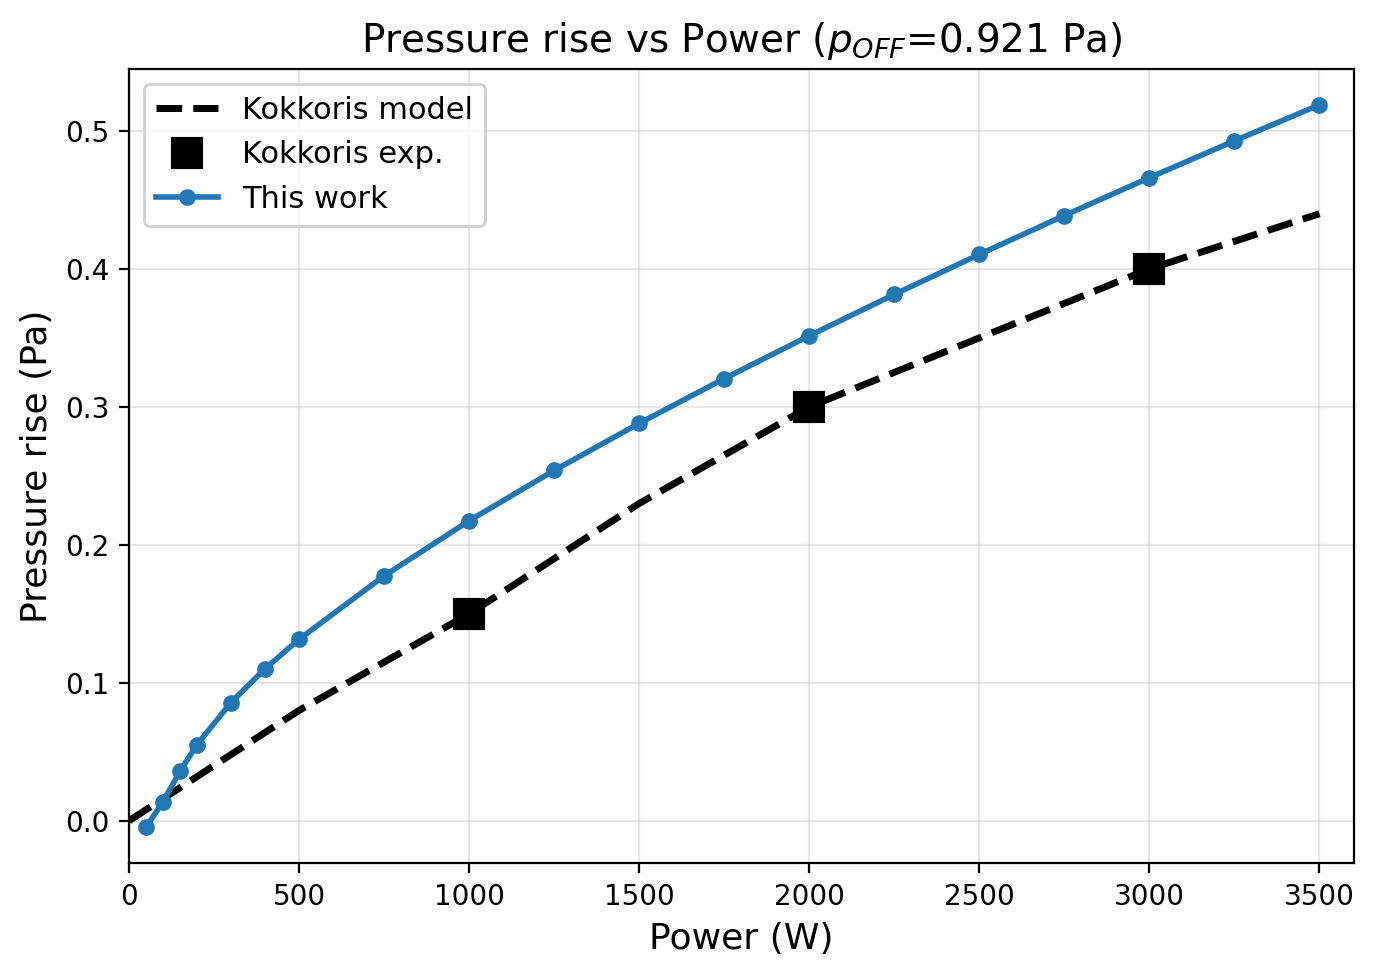
\includegraphics[width=\textwidth]{figs/individual_dp_vs_power.png}
\caption{Pressure rise. Model overestimates by ${\sim}$20\% due to approximate $\eta$. Both sublinear.}
\end{subfigure}\hfill
\begin{subfigure}[t]{0.48\textwidth}
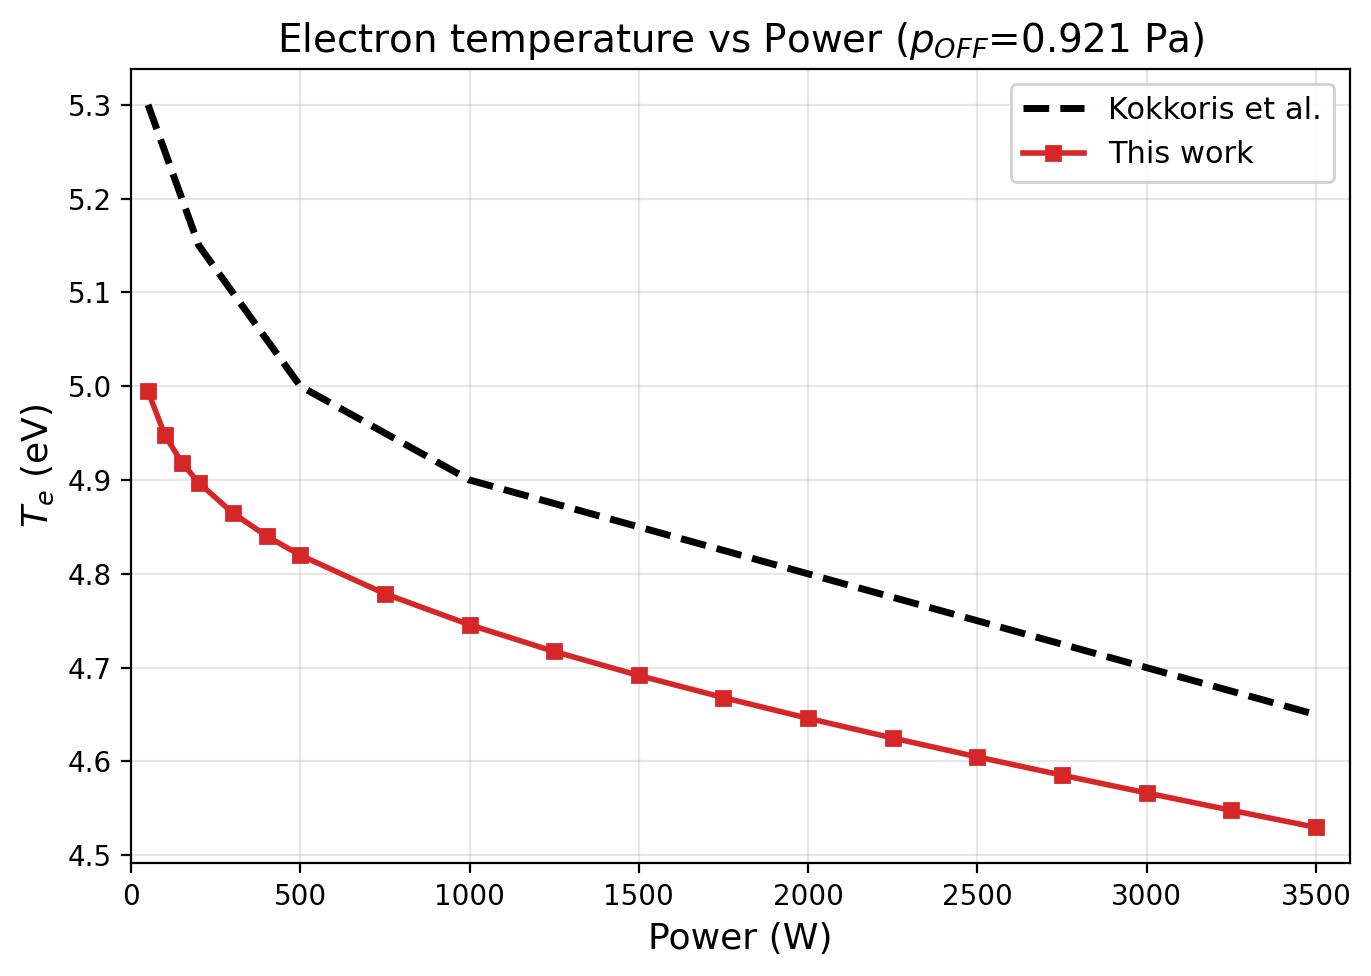
\includegraphics[width=\textwidth]{figs/individual_Te_vs_power.png}
\caption{$T_e$. Offset ${\sim}$0.15\,eV. Same decreasing trend---fragments provide lower ionization thresholds at high power.}
\end{subfigure}
\caption{Pressure rise and electron temperature vs power.}
\end{figure}

\subsection{Neutral Species}

\begin{figure}[H]
\centering
\begin{subfigure}[t]{0.48\textwidth}
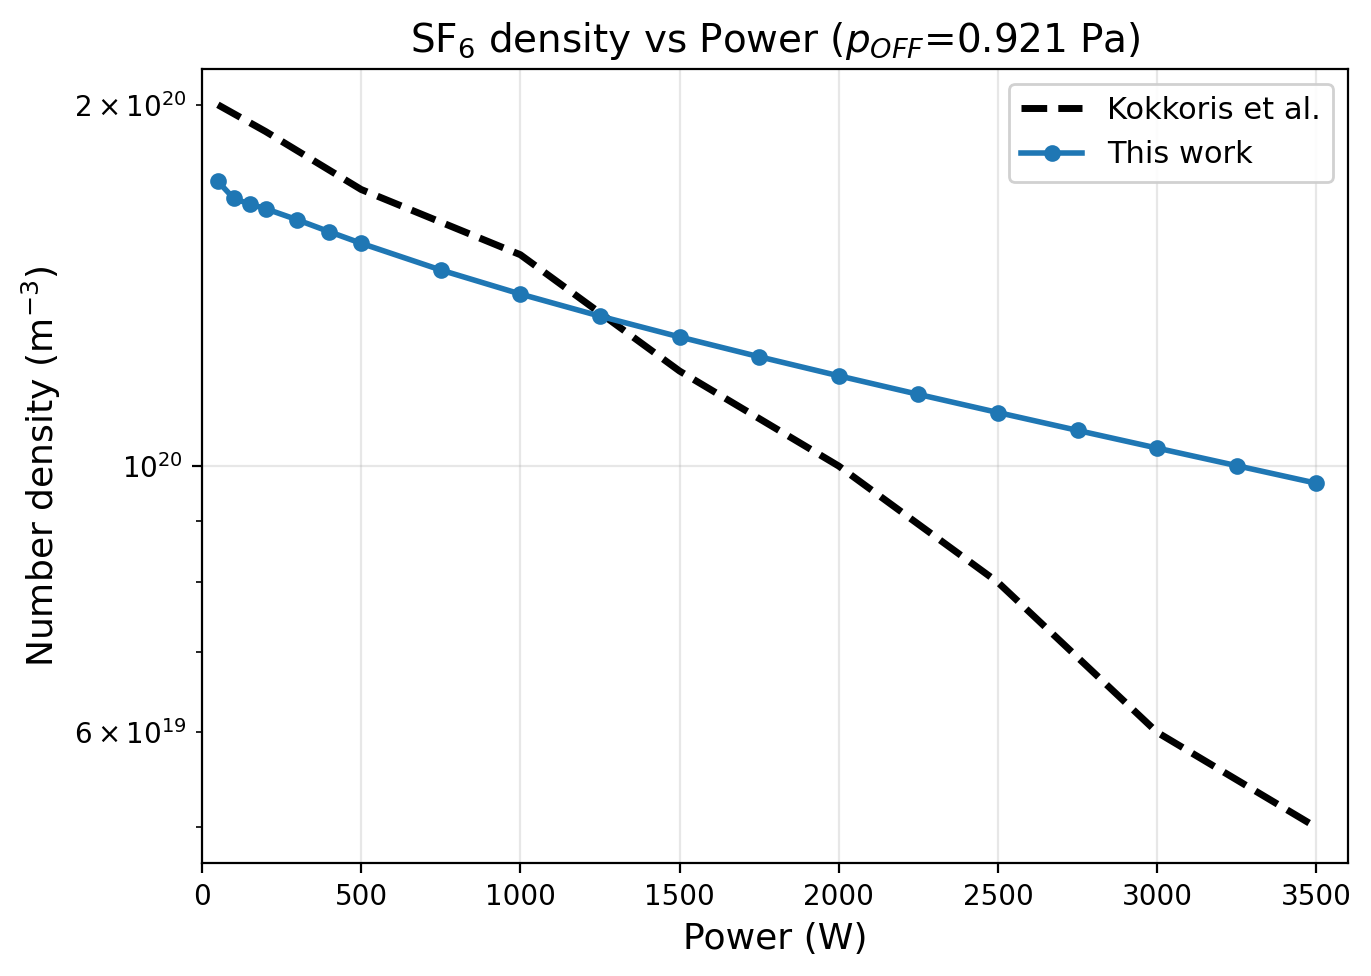
\includegraphics[width=\textwidth]{figs/individual_nSF6_vs_power.png}
\caption{SF$_6$. Both decrease. Our model shows less depletion at high power (lower dissociation from $\eta=0.50$).}
\end{subfigure}\hfill
\begin{subfigure}[t]{0.48\textwidth}
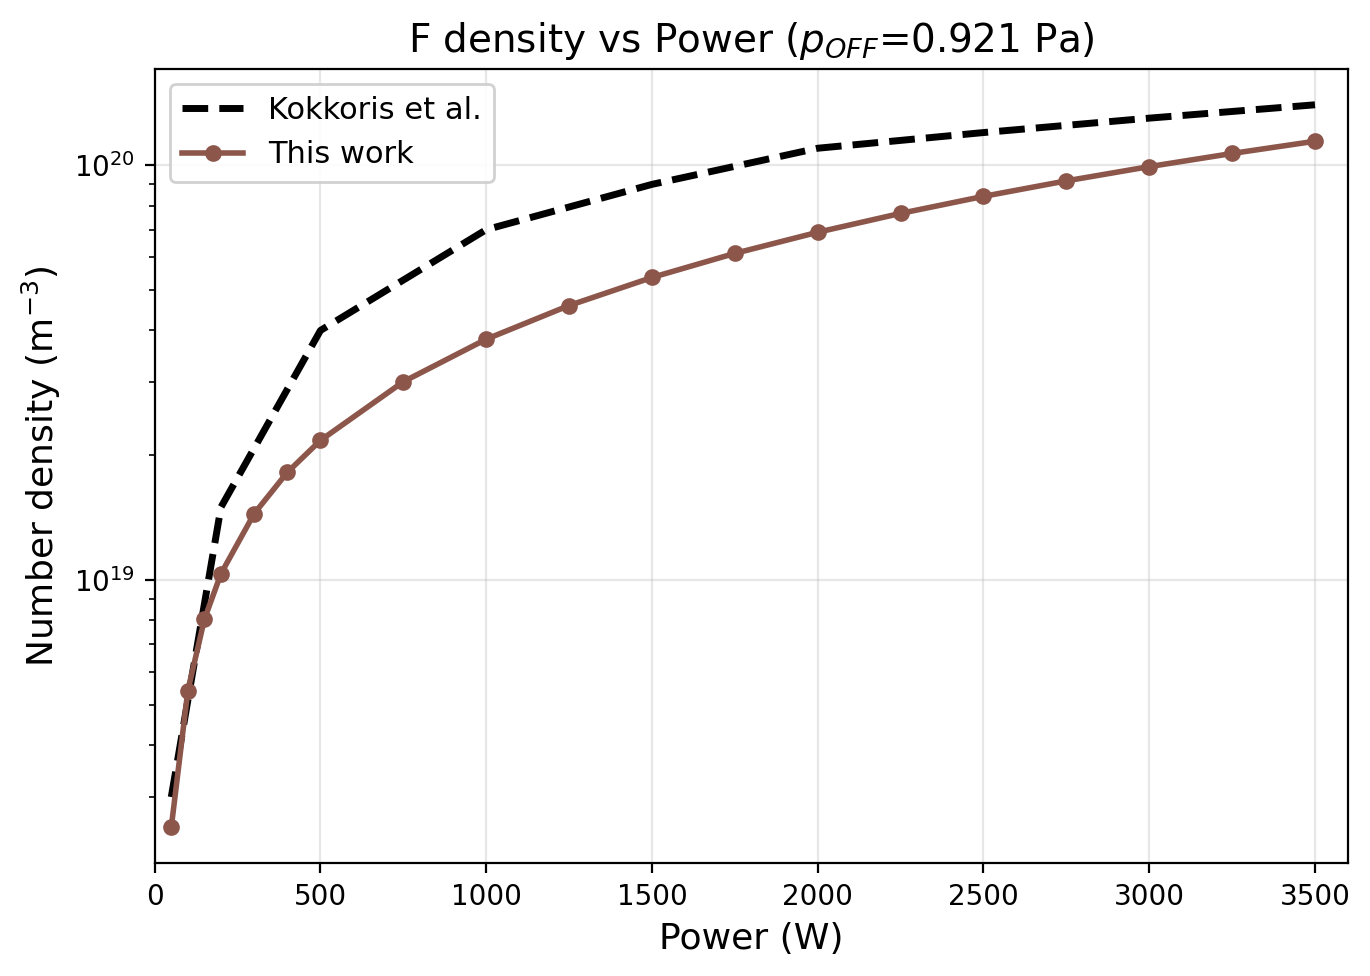
\includegraphics[width=\textwidth]{figs/individual_nF_vs_power.png}
\caption{F. Both increase linearly. Our density ${\sim}$0.5--0.7$\times$.}
\end{subfigure}
\caption{SF$_6$ and F vs power.}
\end{figure}

\begin{figure}[H]
\centering
\begin{subfigure}[t]{0.48\textwidth}
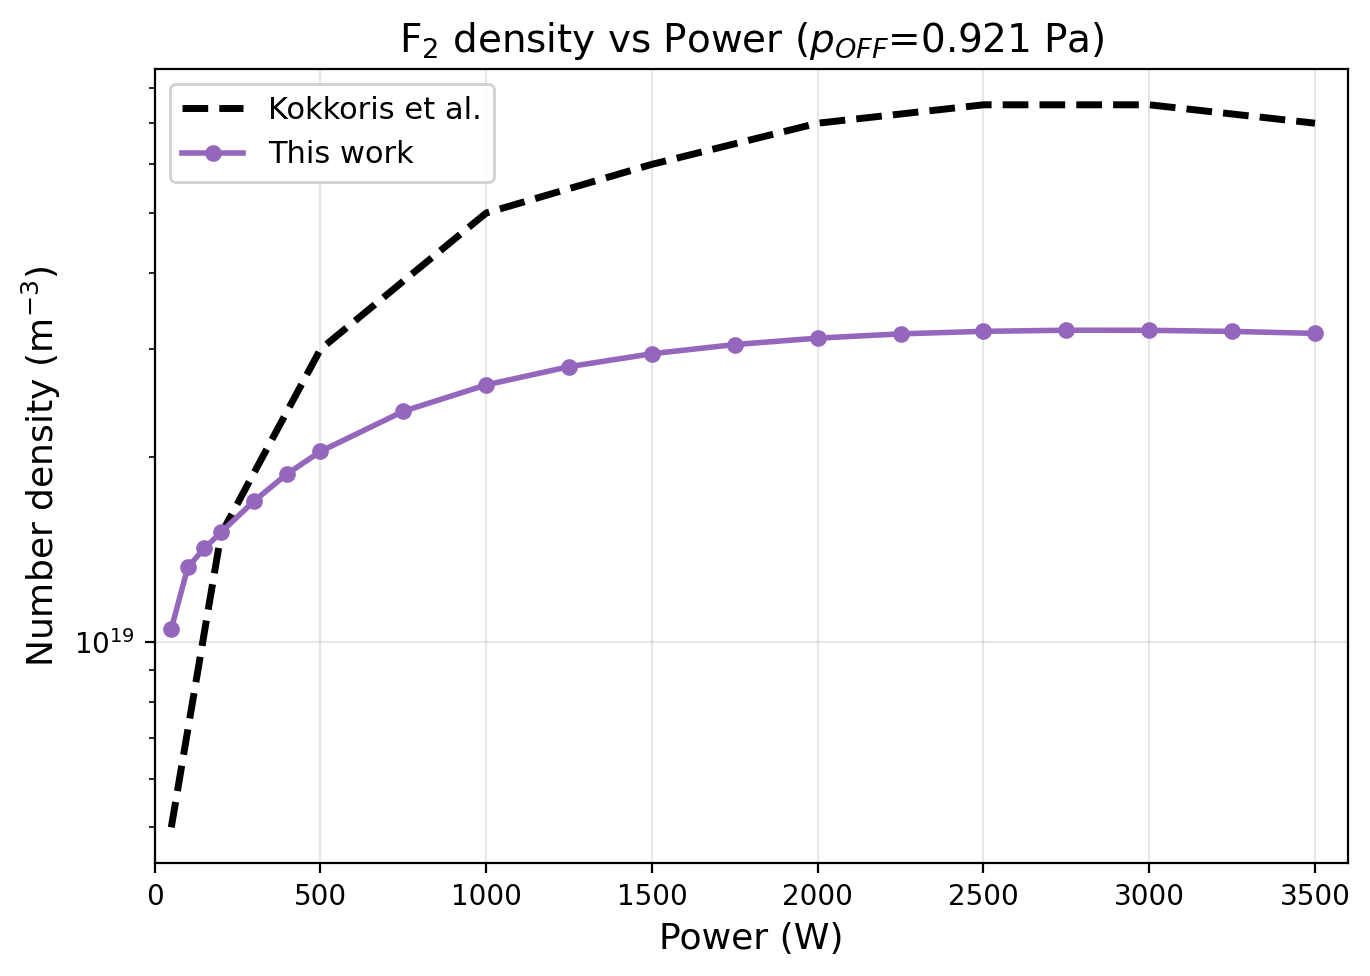
\includegraphics[width=\textwidth]{figs/individual_nF2_vs_power.png}
\caption{F$_2$. Both saturate. Our value ${\sim}$0.5$\times$ because F$_2$ is produced from F surface recombination (S8).}
\end{subfigure}\hfill
\begin{subfigure}[t]{0.48\textwidth}
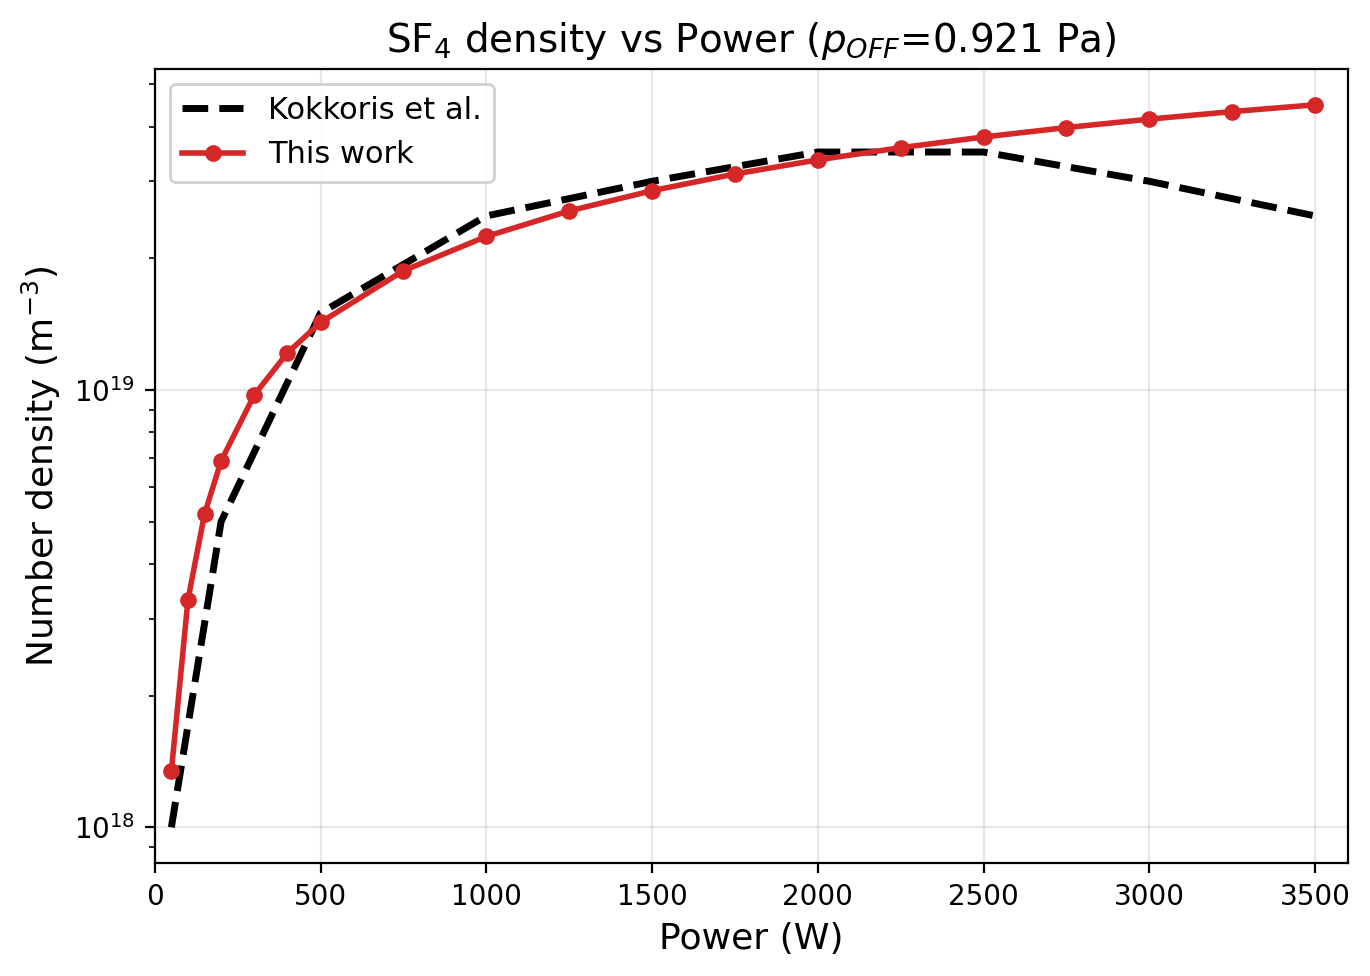
\includegraphics[width=\textwidth]{figs/individual_nSF4_vs_power.png}
\caption{SF$_4$. Both increase. Match within 1.5$\times$.}
\end{subfigure}
\caption{F$_2$ and SF$_4$ vs power.}
\end{figure}

\begin{figure}[H]
\centering
\begin{subfigure}[t]{0.48\textwidth}
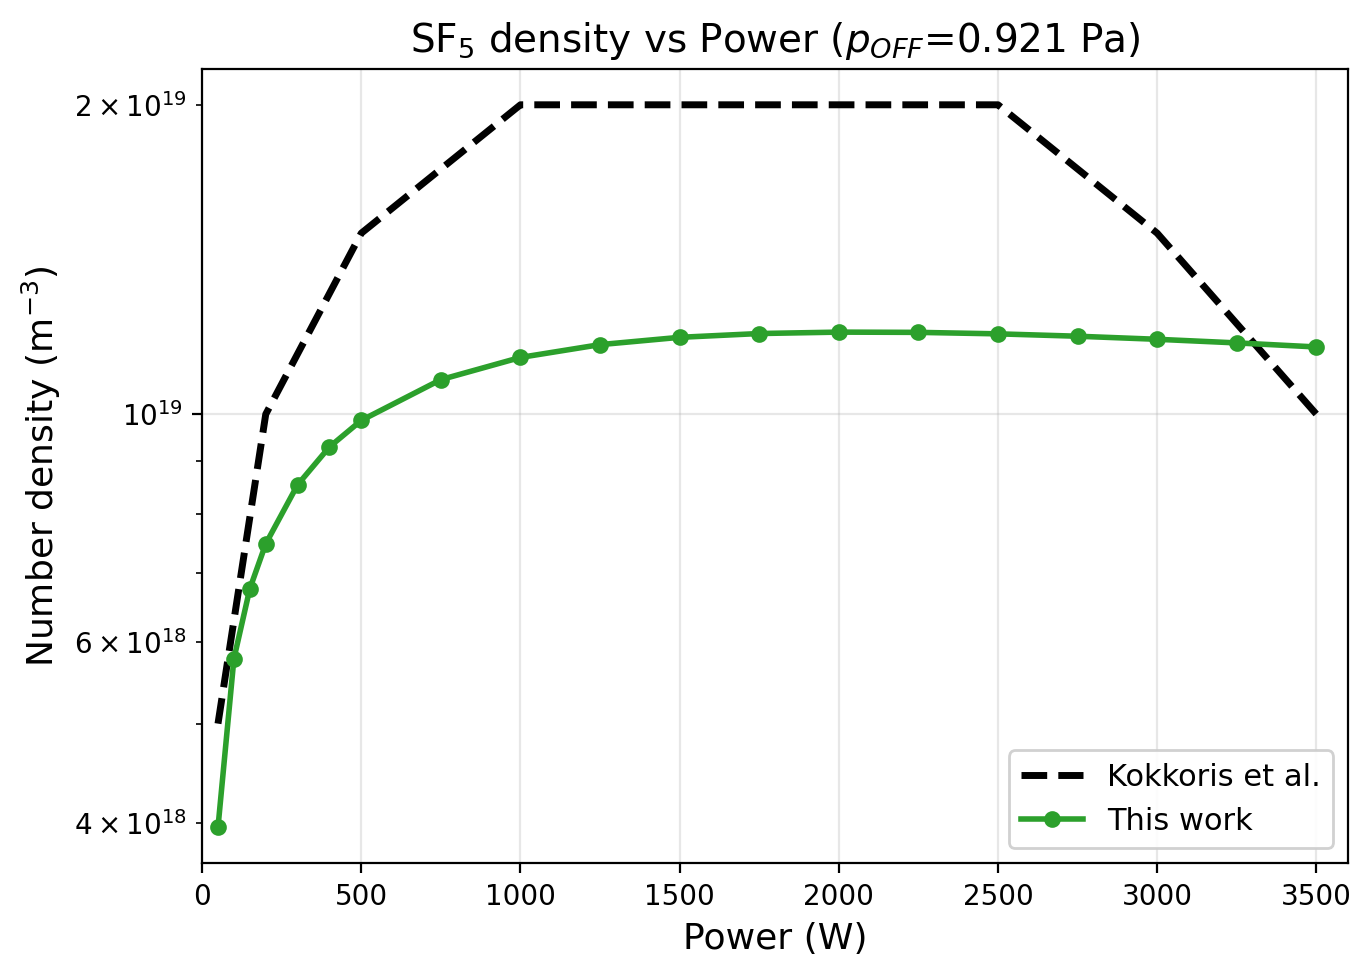
\includegraphics[width=\textwidth]{figs/individual_nSF5_vs_power.png}
\caption{SF$_5$. Both flat ${\sim}10^{19}$\,m$^{-3}$ due to Troe recombination buffer (G35). Match within 0.5--0.7$\times$.}
\end{subfigure}\hfill
\begin{subfigure}[t]{0.48\textwidth}
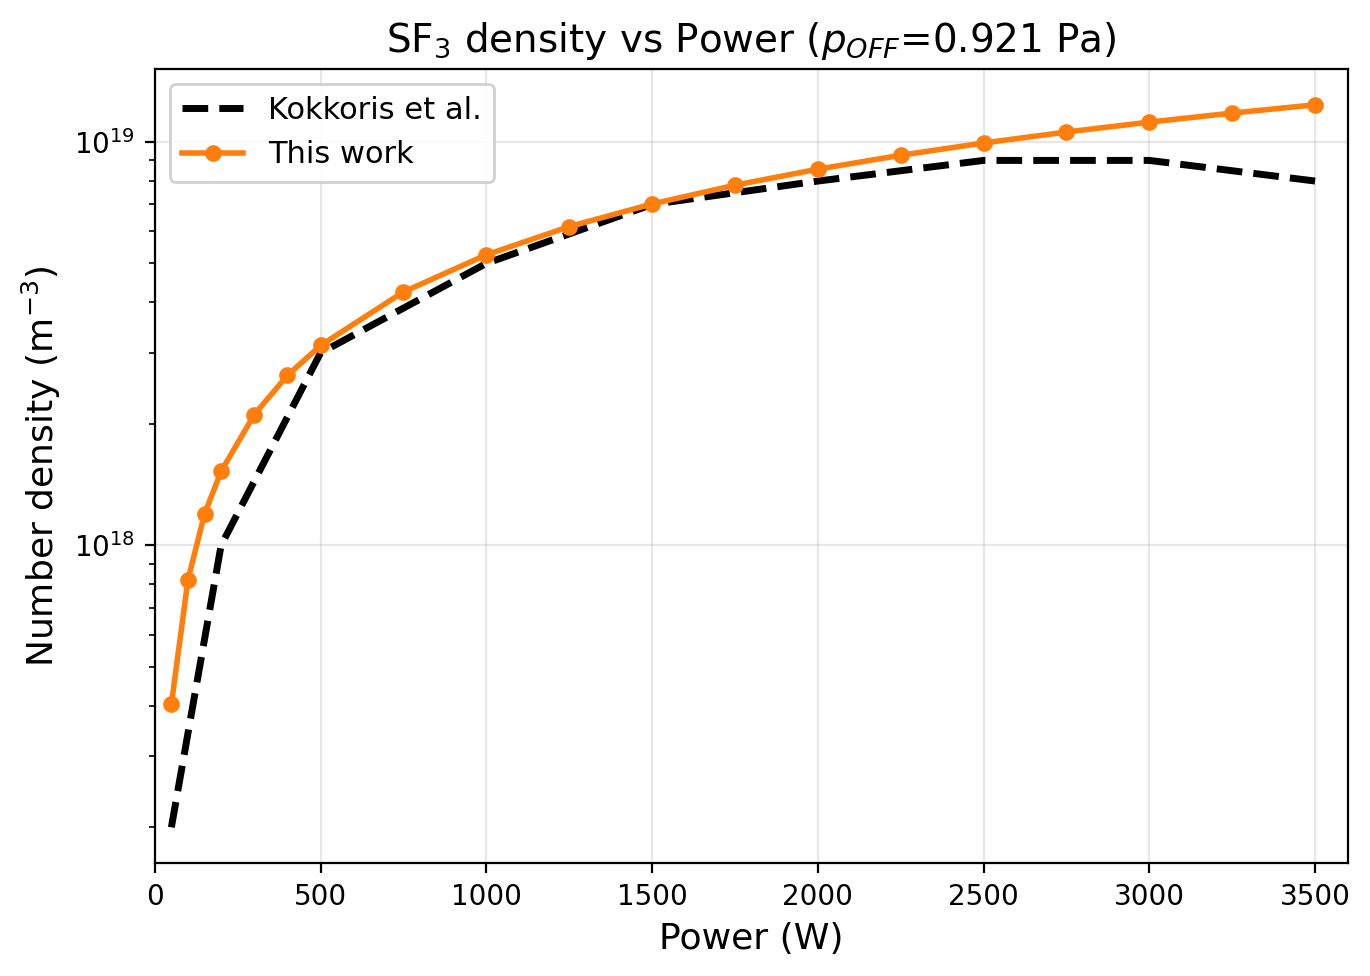
\includegraphics[width=\textwidth]{figs/individual_nSF3_vs_power.png}
\caption{SF$_3$. Both increase. Lowest radical in both models.}
\end{subfigure}
\caption{SF$_5$ and SF$_3$ vs power.}
\end{figure}

\subsection{Charged Species and Electronegativity}

\begin{figure}[H]
\centering
\begin{subfigure}[t]{0.48\textwidth}
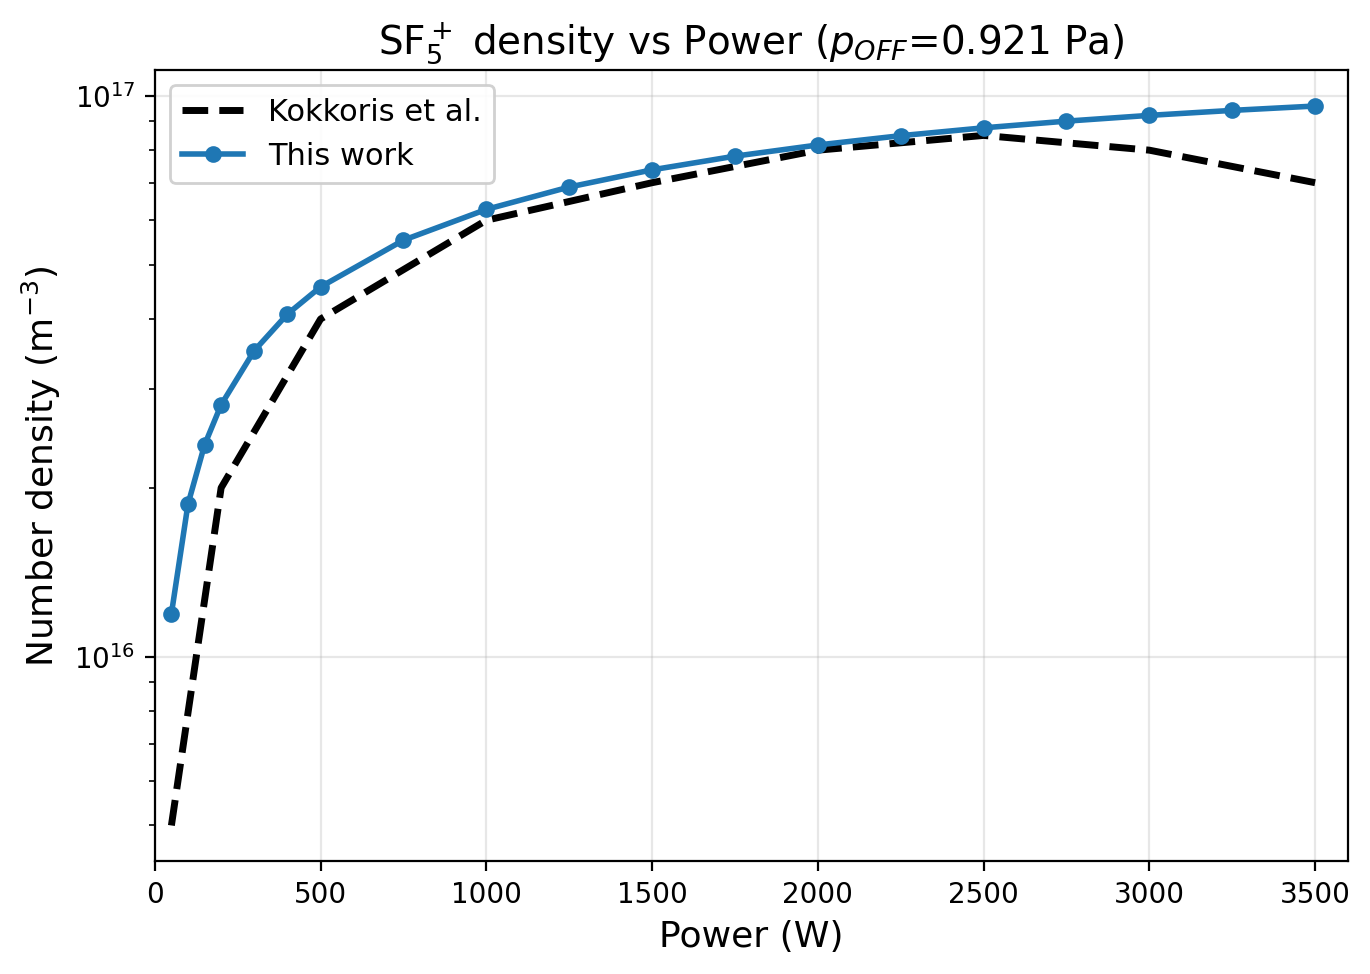
\includegraphics[width=\textwidth]{figs/individual_nSF5p_vs_power.png}
\caption{SF$_5^+$. Dominant positive ion in both. Within 2$\times$.}
\end{subfigure}\hfill
\begin{subfigure}[t]{0.48\textwidth}
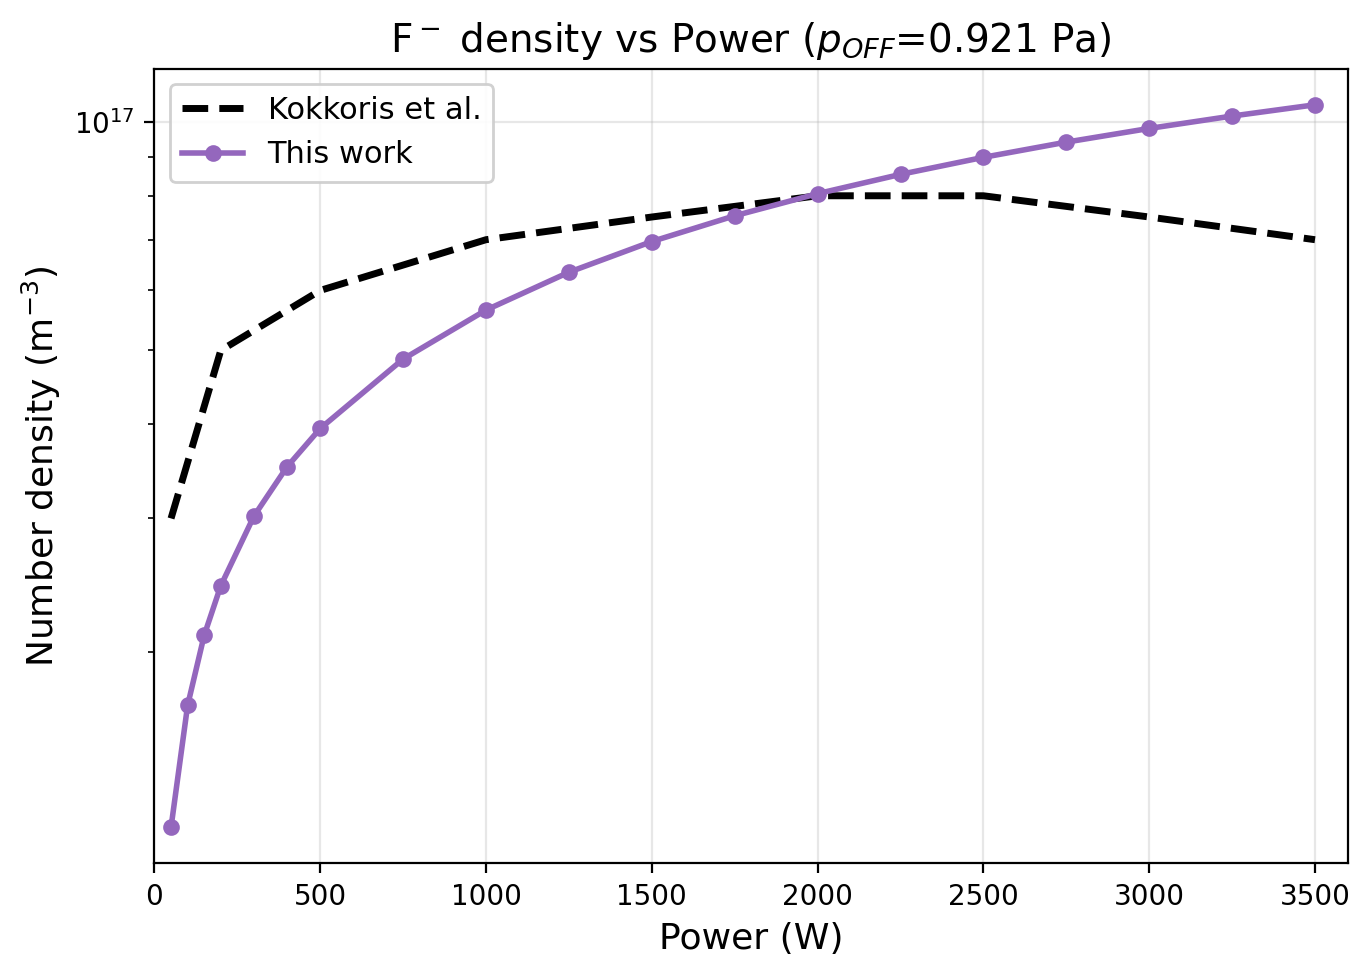
\includegraphics[width=\textwidth]{figs/individual_nFm_vs_power.png}
\caption{F$^-$. Dominant negative ion in both. Excellent match.}
\end{subfigure}
\caption{Dominant ions vs power.}
\end{figure}

\begin{figure}[H]
\centering
\begin{subfigure}[t]{0.48\textwidth}
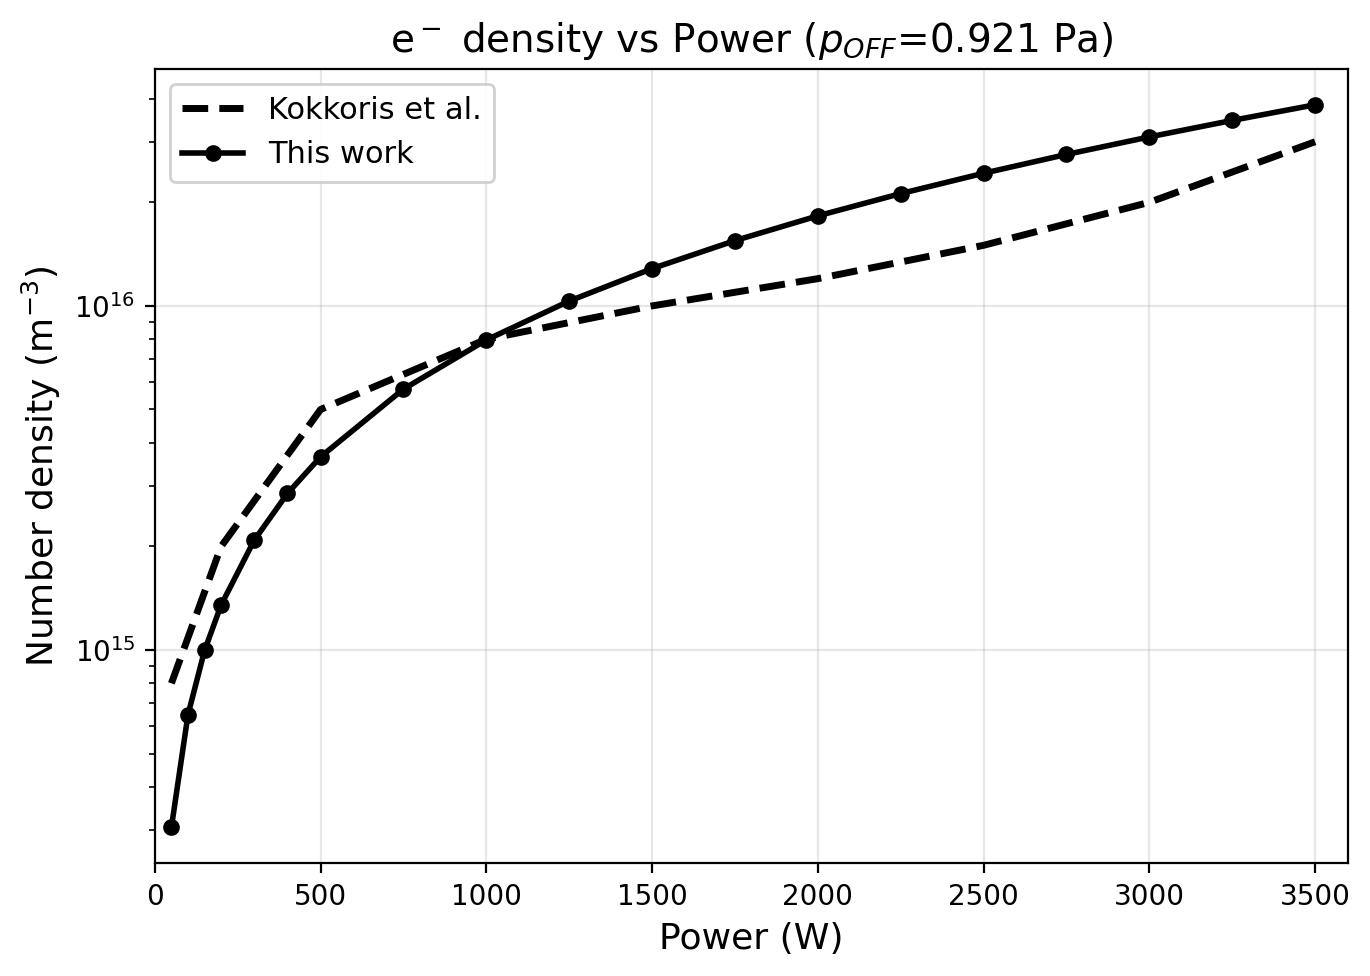
\includegraphics[width=\textwidth]{figs/individual_ne_vs_power.png}
\caption{$n_e$. Both increase. Our $n_e$ is ${\sim}$1.5--2$\times$ higher.}
\end{subfigure}\hfill
\begin{subfigure}[t]{0.48\textwidth}
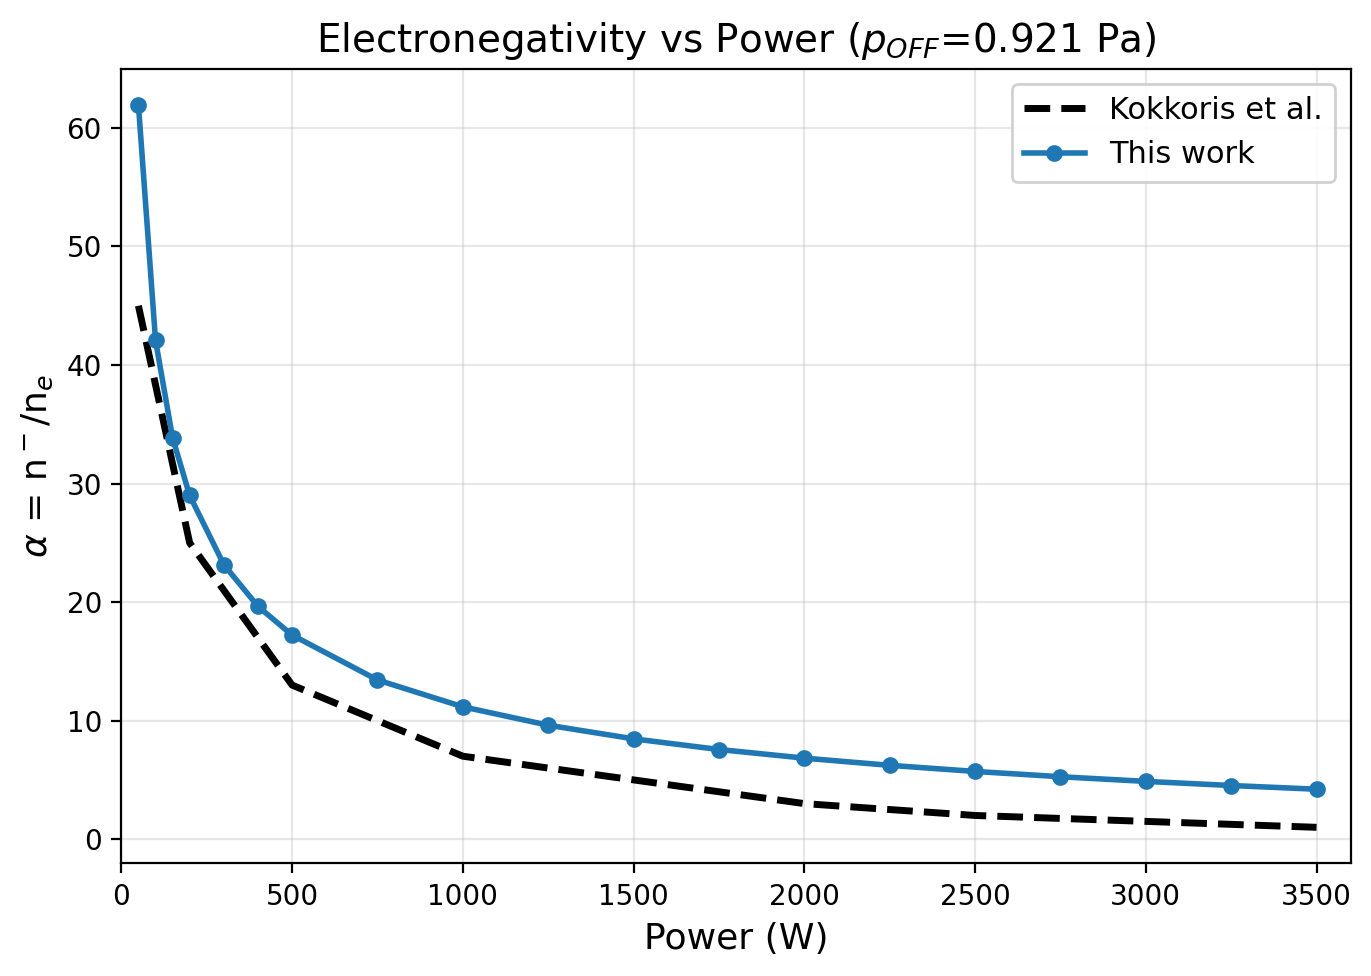
\includegraphics[width=\textwidth]{figs/individual_alpha_vs_power.png}
\caption{$\alpha$. Hyperbolic in both. Our values ${\sim}$2--3$\times$ higher due to h-factor interpolation.}
\end{subfigure}
\caption{$n_e$ and $\alpha$ vs power.}
\end{figure}

\subsection{Densities vs Electron Temperature}

\begin{figure}[H]
\centering
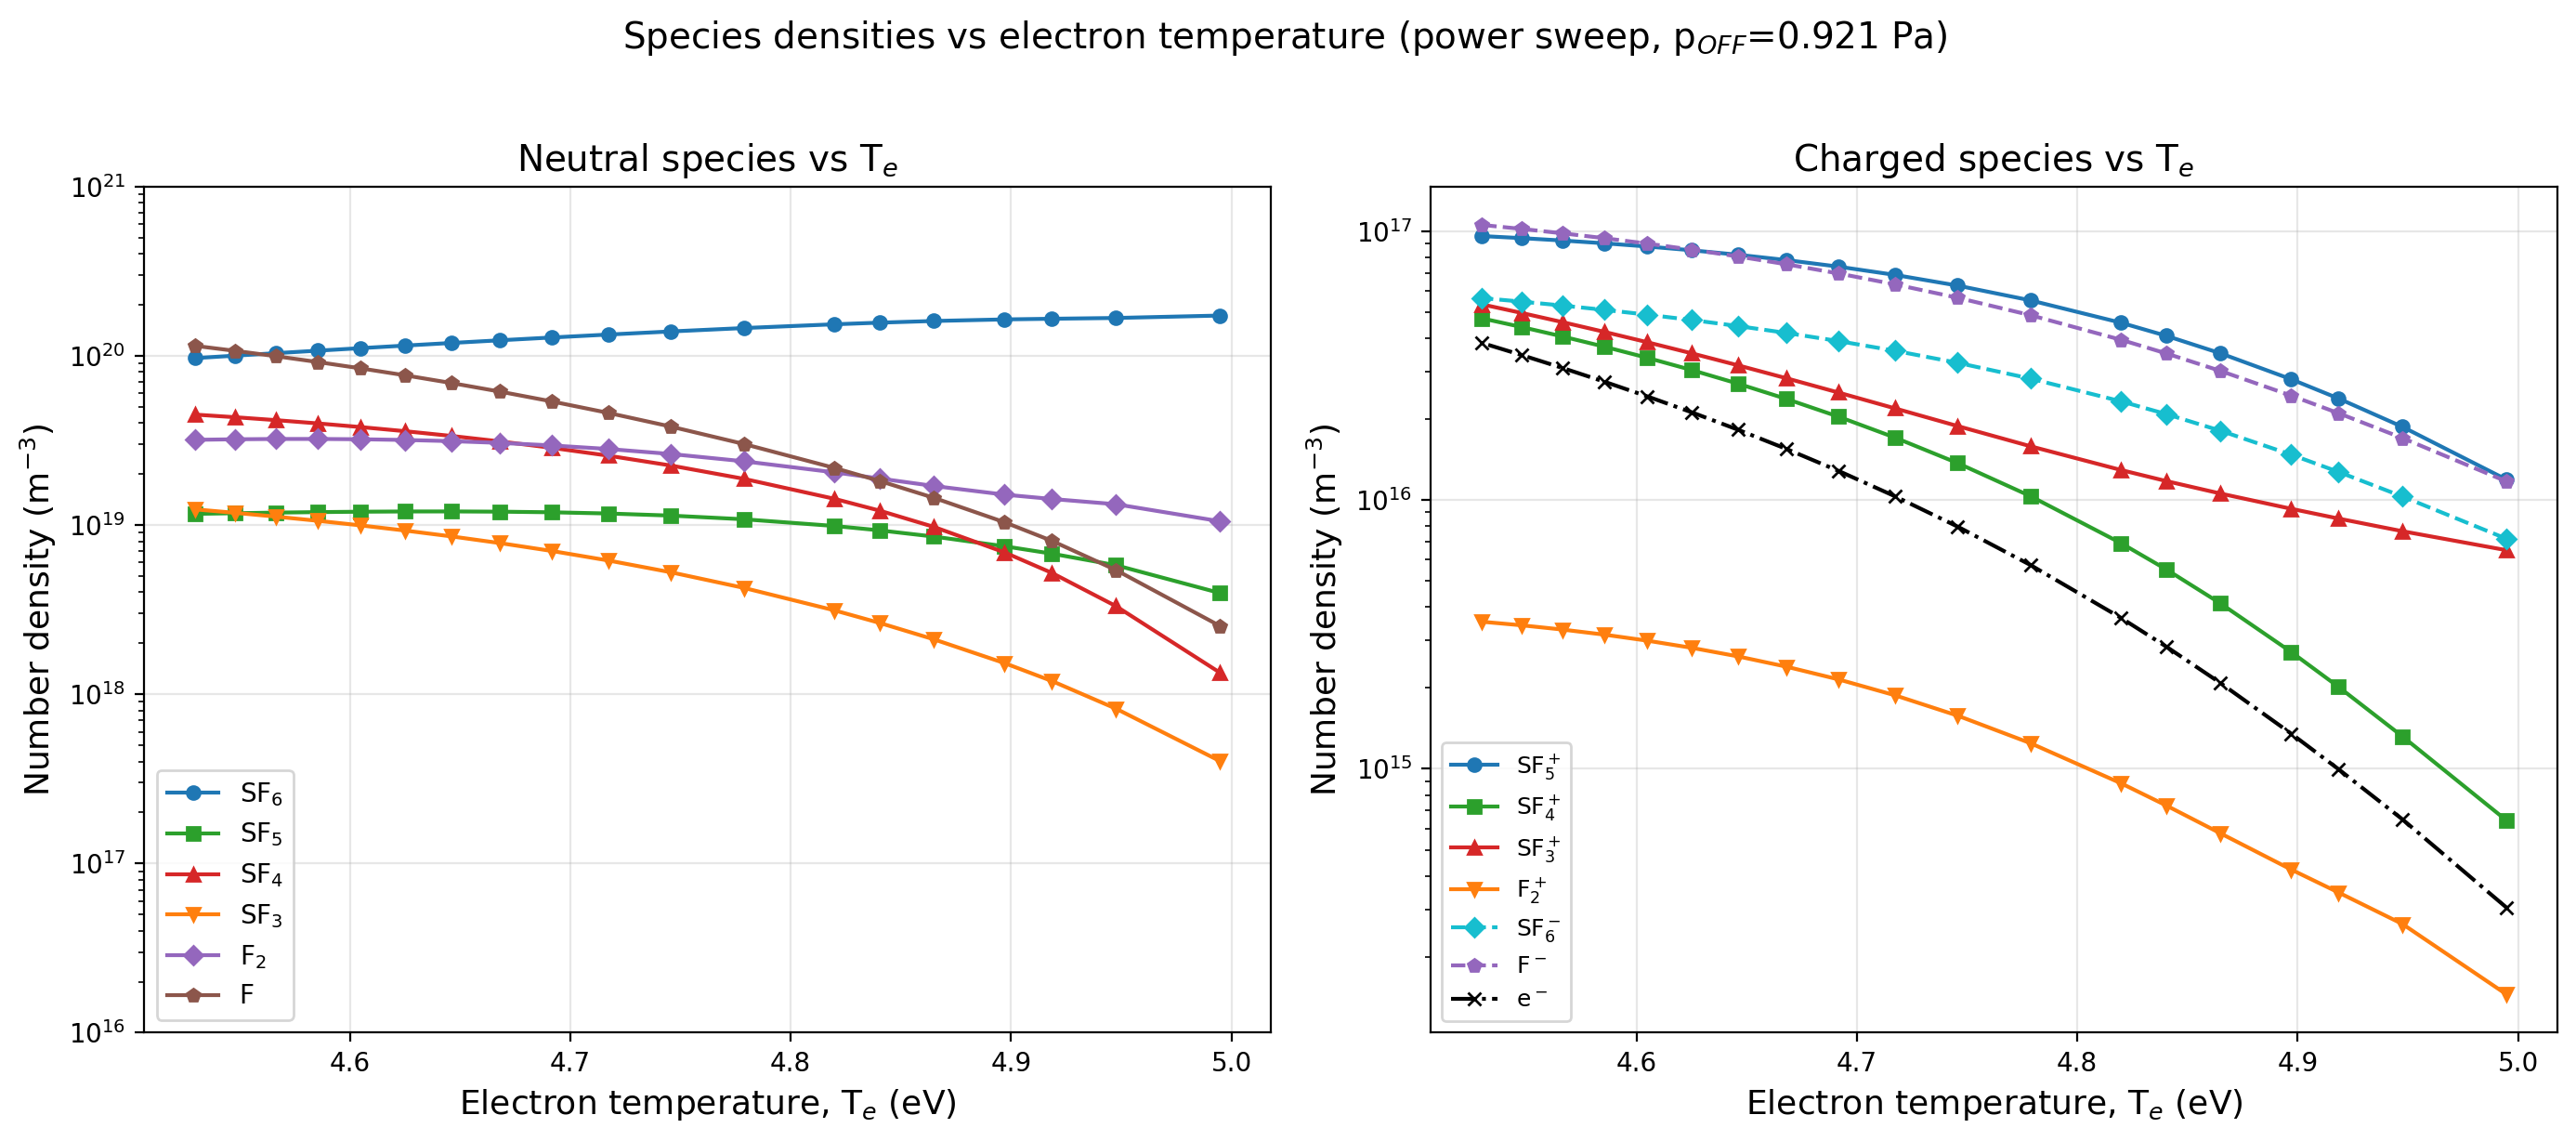
\includegraphics[width=0.95\textwidth]{figs/model_densities_Te_power.png}
\caption{Species densities vs $T_e$ from the power sweep (no paper equivalent). $T_e$ ranges 4.5--5.0\,eV; a 0.5\,eV change produces order-of-magnitude changes in species composition through the exponential dependence of rate coefficients.}
\end{figure}

\section{Pressure Sweep ($P = 2000$\,W, 13 points)}

\subsection{Pressure Rise and Electron Temperature}

\begin{figure}[H]
\centering
\begin{subfigure}[t]{0.48\textwidth}
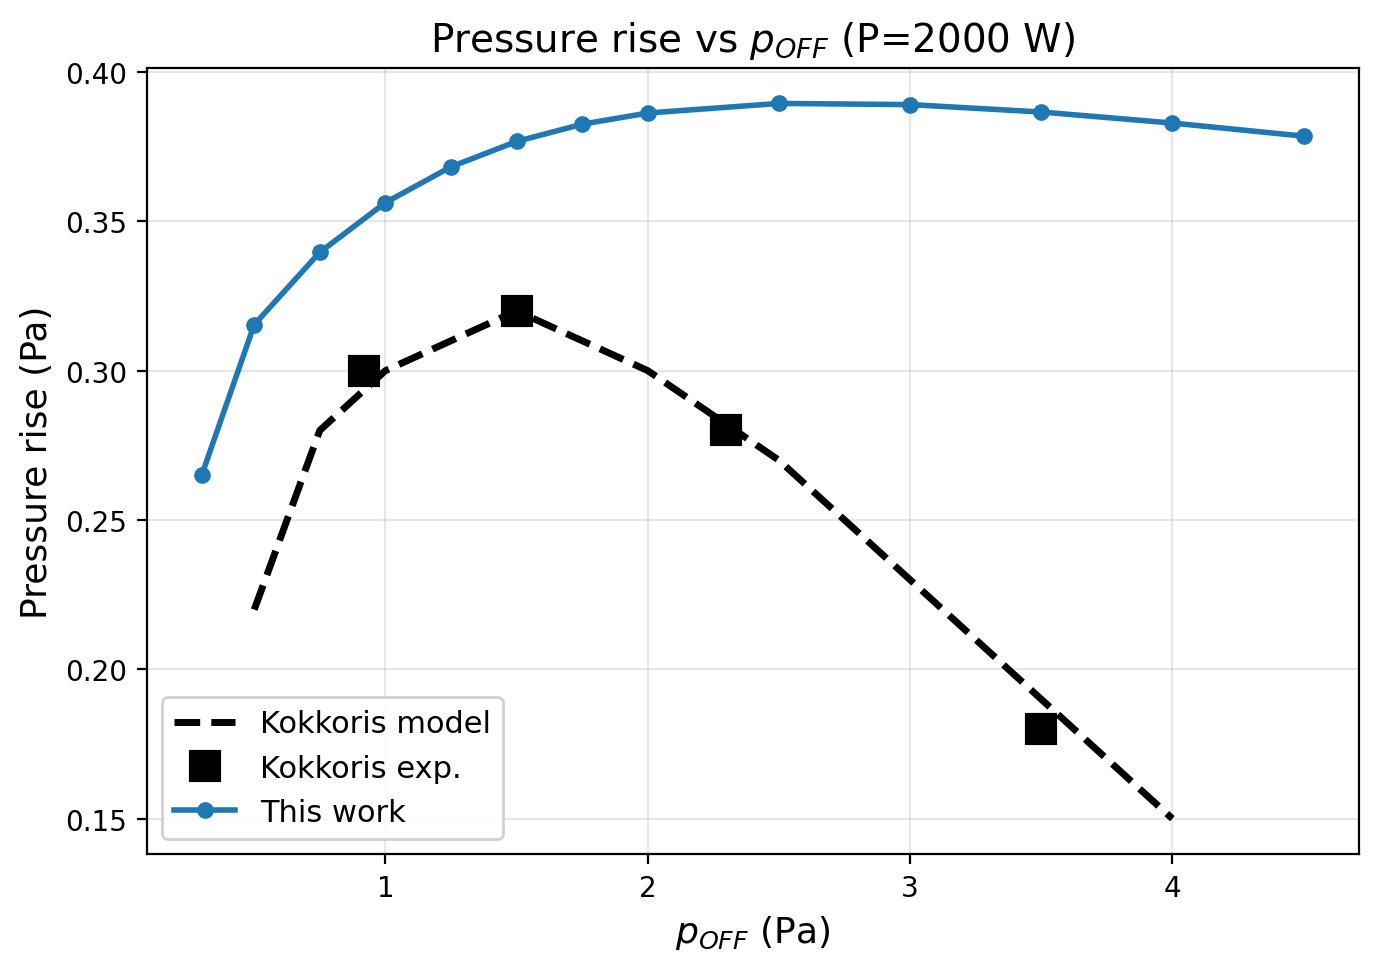
\includegraphics[width=\textwidth]{figs/individual_dp_vs_poff.png}
\caption{Pressure rise. Both show the turnover due to SF$_x$ deposition. Peak shifted slightly in our model.}
\end{subfigure}\hfill
\begin{subfigure}[t]{0.48\textwidth}
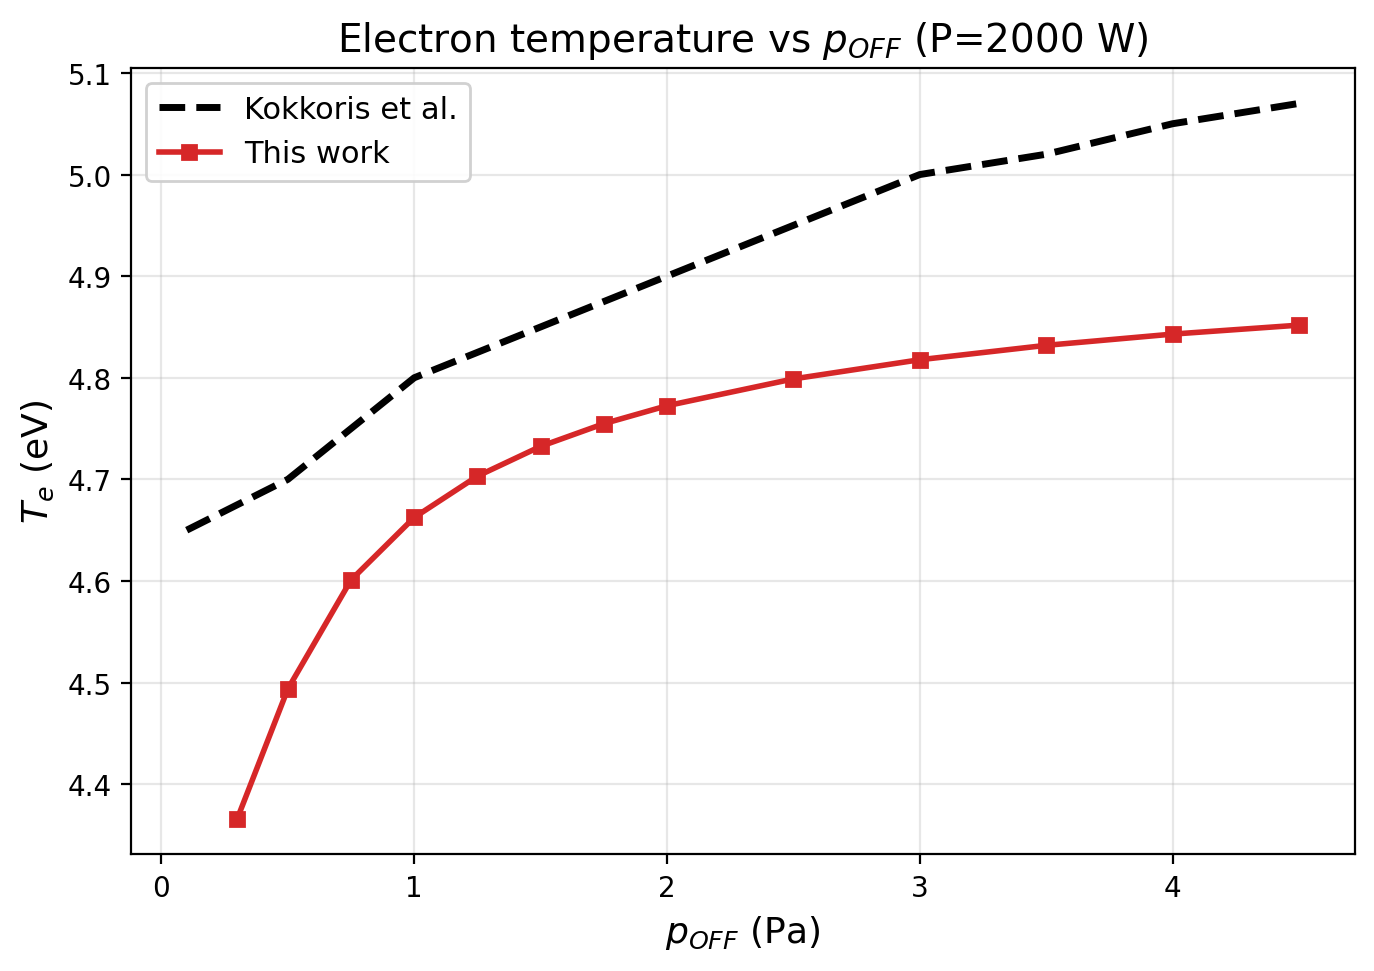
\includegraphics[width=\textwidth]{figs/individual_Te_vs_poff.png}
\caption{$T_e$. Both increase with pressure. Offset ${\sim}$0.2\,eV, consistent with power sweep.}
\end{subfigure}
\caption{Pressure rise and $T_e$ vs $p_\text{OFF}$.}
\end{figure}

\subsection{Neutral Species}

\begin{figure}[H]
\centering
\begin{subfigure}[t]{0.48\textwidth}
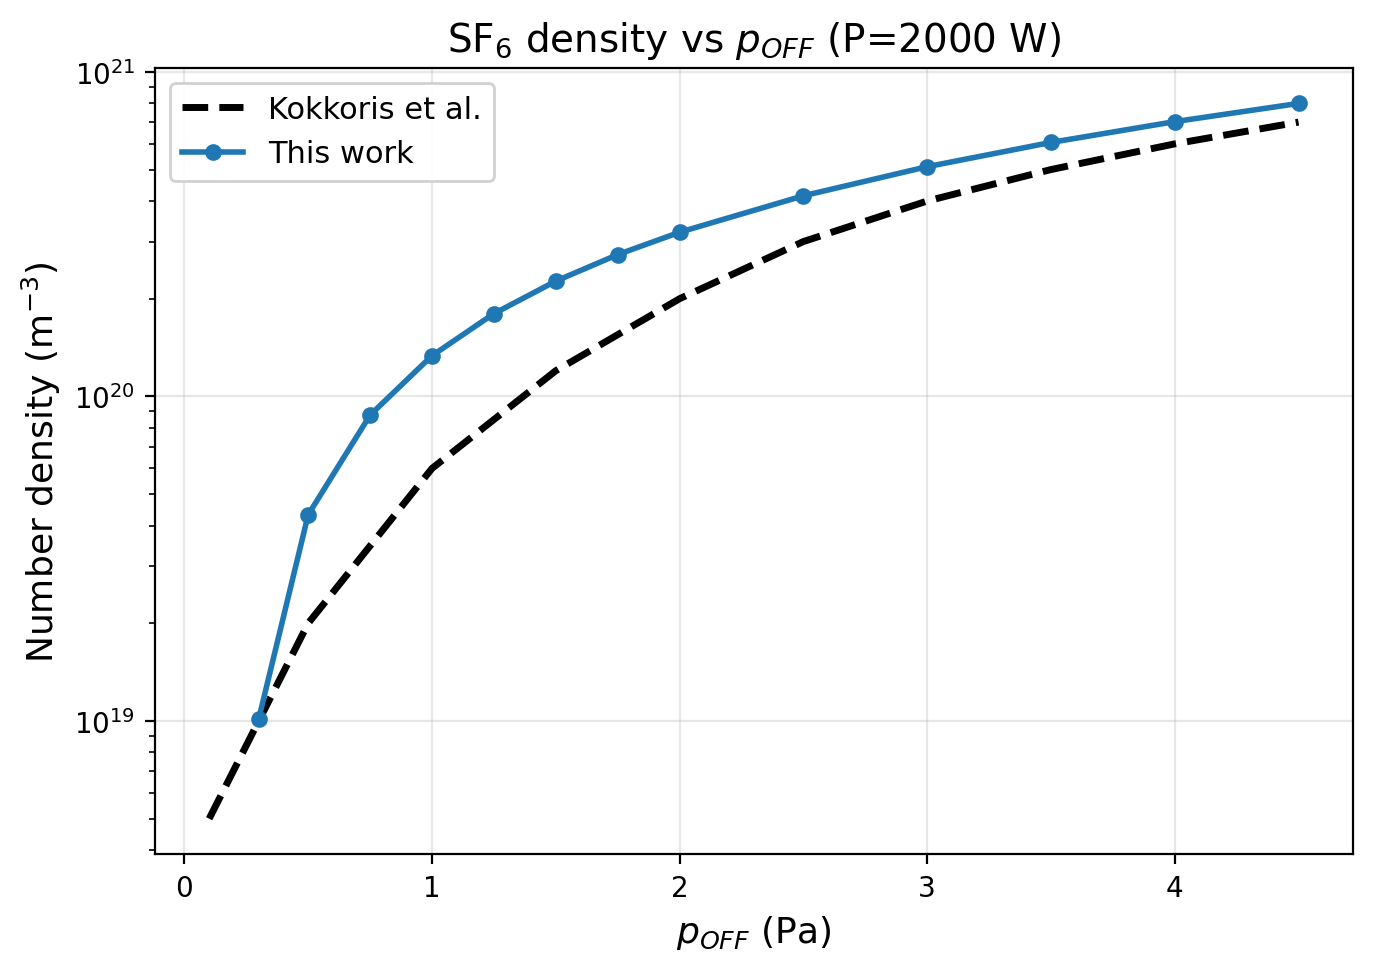
\includegraphics[width=\textwidth]{figs/individual_nSF6_vs_poff.png}
\caption{SF$_6$. Both increase steeply. Within 1.5$\times$.}
\end{subfigure}\hfill
\begin{subfigure}[t]{0.48\textwidth}
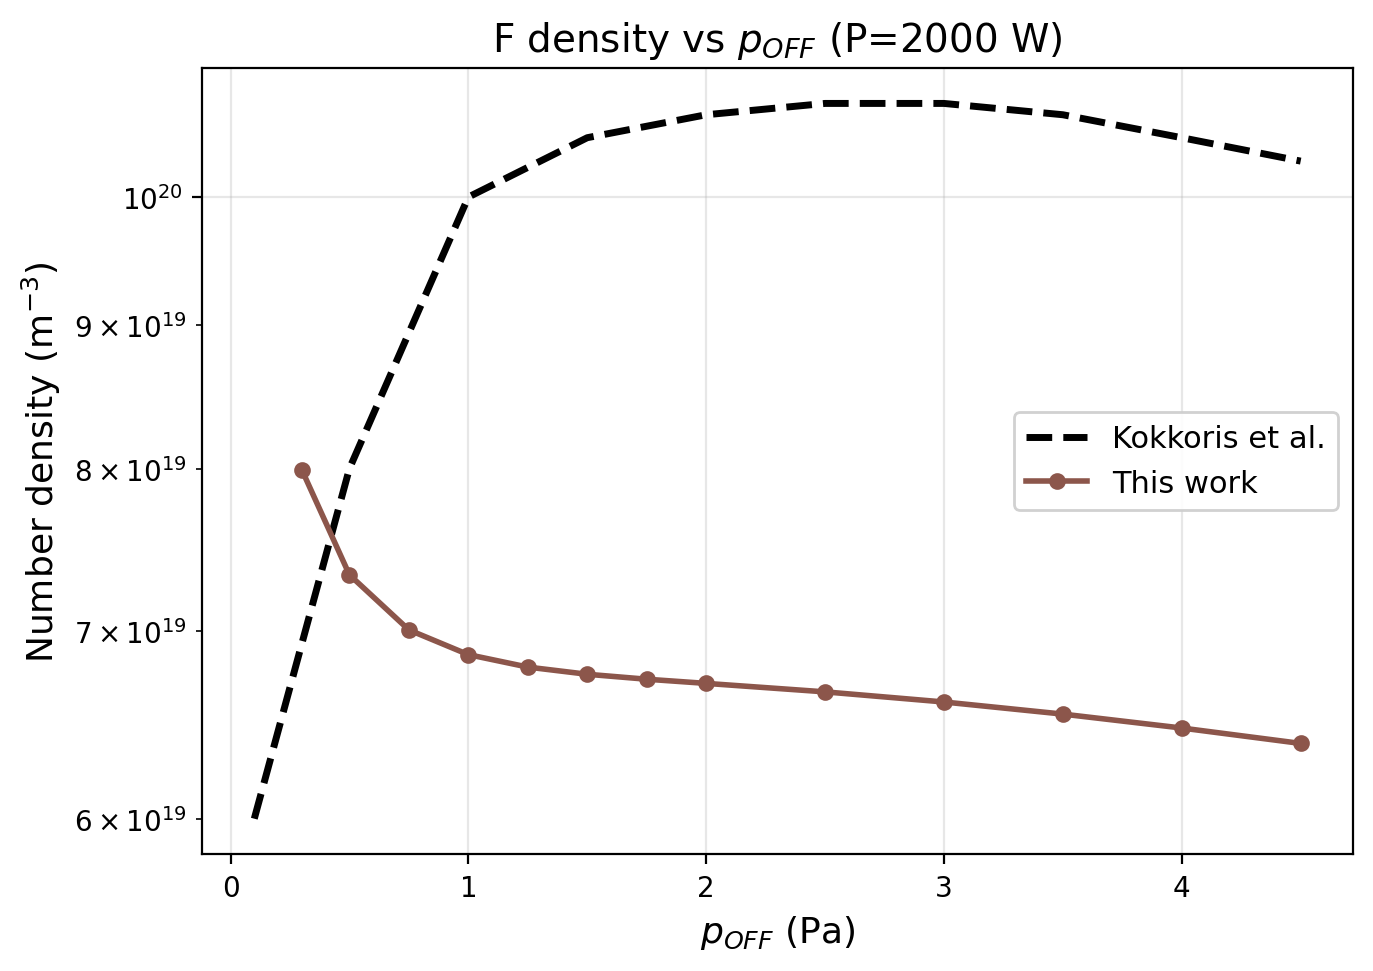
\includegraphics[width=\textwidth]{figs/individual_nF_vs_poff.png}
\caption{F. Both decrease. Our density ${\sim}$0.7$\times$.}
\end{subfigure}
\caption{SF$_6$ and F vs $p_\text{OFF}$.}
\end{figure}

\begin{figure}[H]
\centering
\begin{subfigure}[t]{0.48\textwidth}
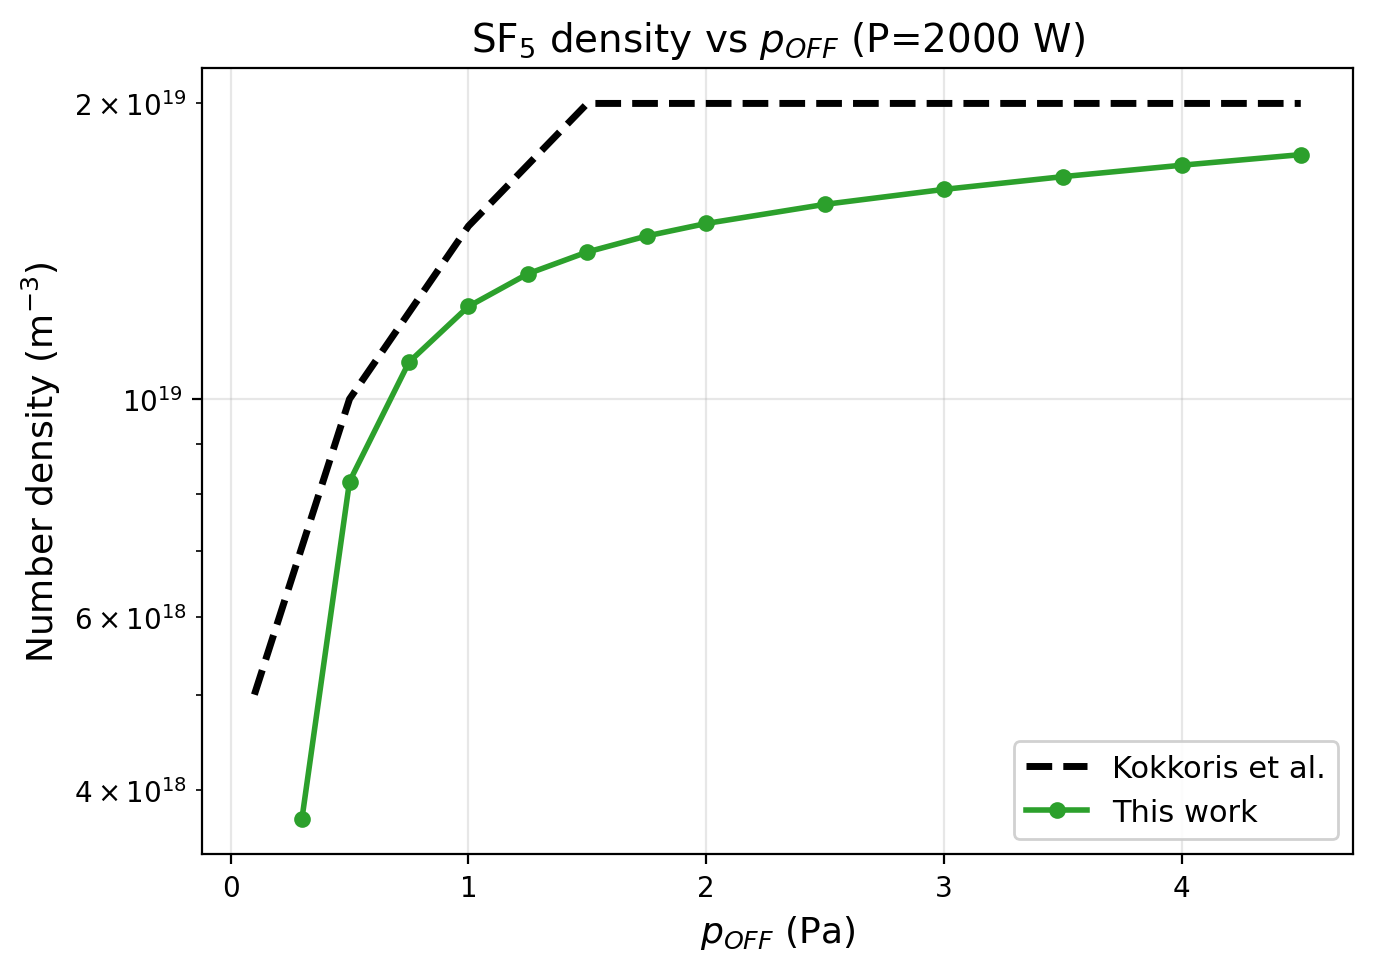
\includegraphics[width=\textwidth]{figs/individual_nSF5_vs_poff.png}
\caption{SF$_5$. Both flat at ${\sim}10^{19}$\,m$^{-3}$. Within 30\%---best match.}
\end{subfigure}\hfill
\begin{subfigure}[t]{0.48\textwidth}
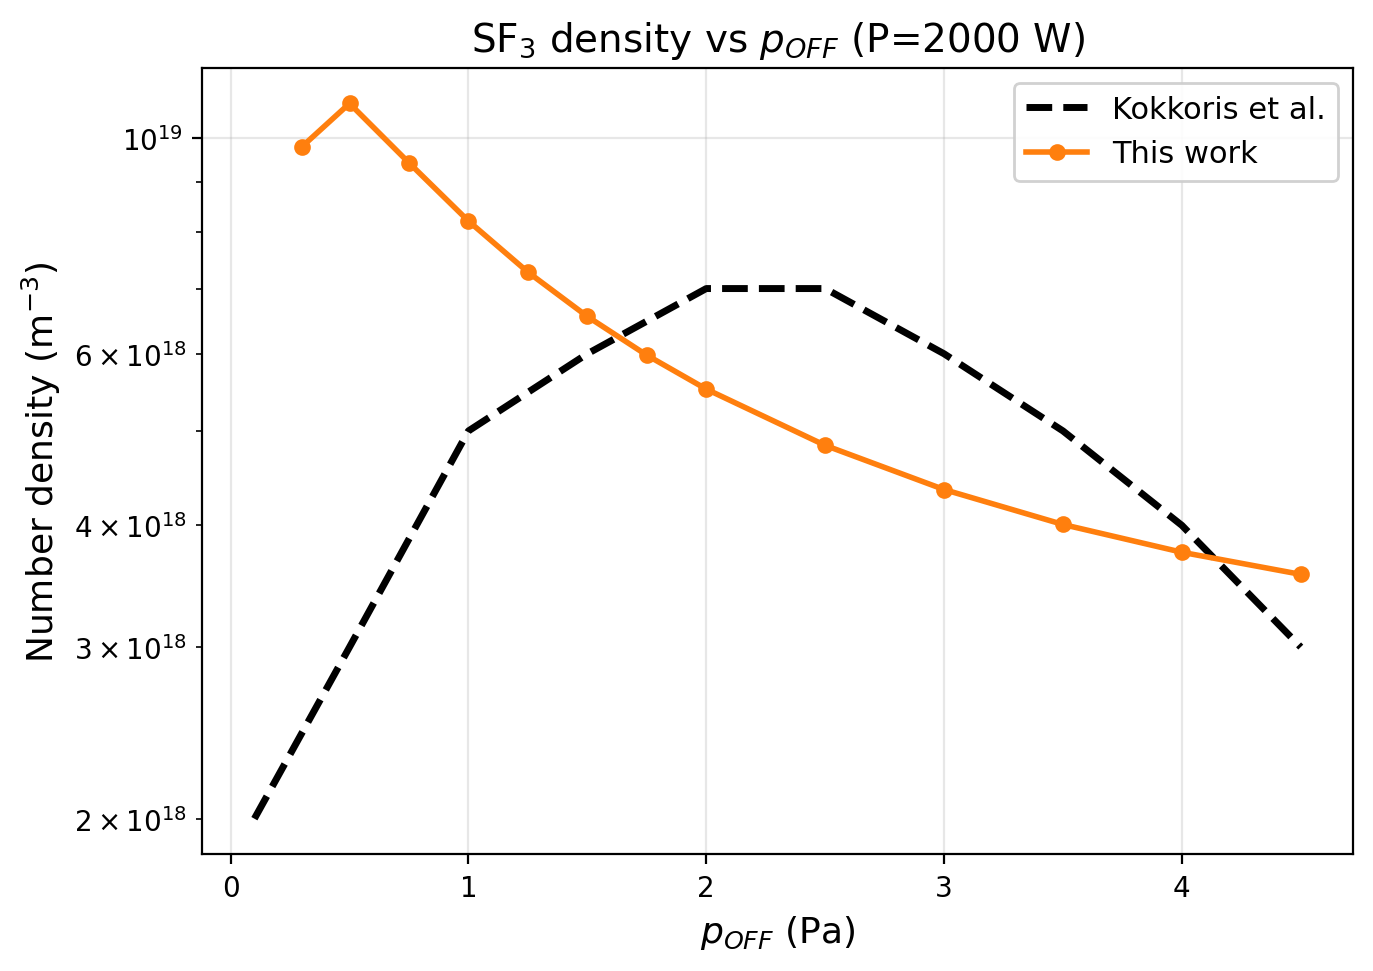
\includegraphics[width=\textwidth]{figs/individual_nSF3_vs_poff.png}
\caption{SF$_3$. Both decrease at high pressure.}
\end{subfigure}
\caption{SF$_5$ and SF$_3$ vs $p_\text{OFF}$.}
\end{figure}

\subsection{Electron Density and Electronegativity}

\begin{figure}[H]
\centering
\begin{subfigure}[t]{0.48\textwidth}
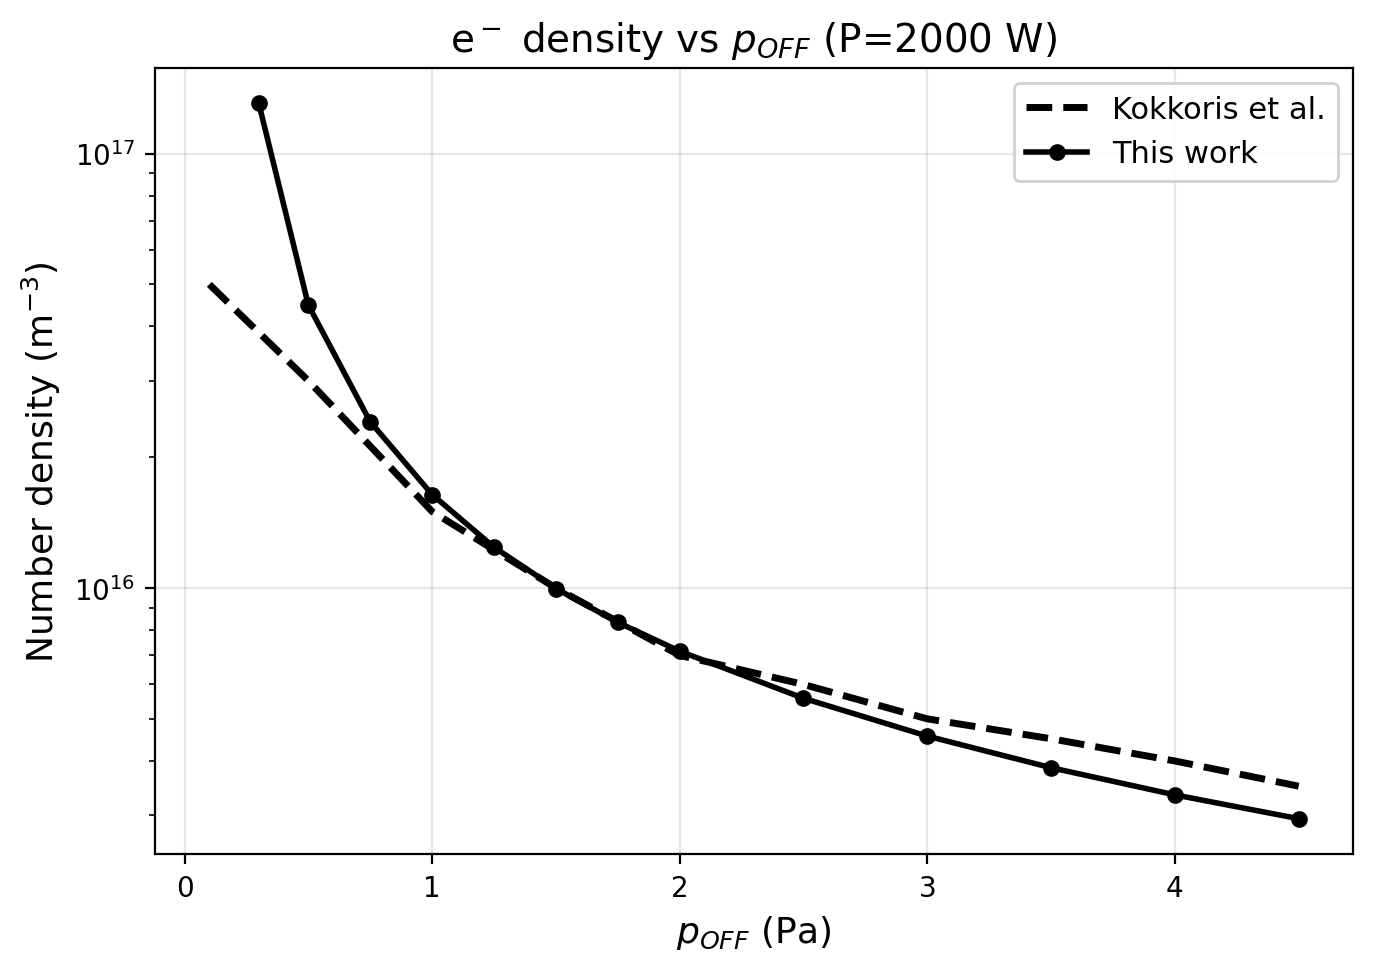
\includegraphics[width=\textwidth]{figs/individual_ne_vs_poff.png}
\caption{$n_e$. Both drop by $>$10$\times$ from 0.5 to 4.5\,Pa.}
\end{subfigure}\hfill
\begin{subfigure}[t]{0.48\textwidth}
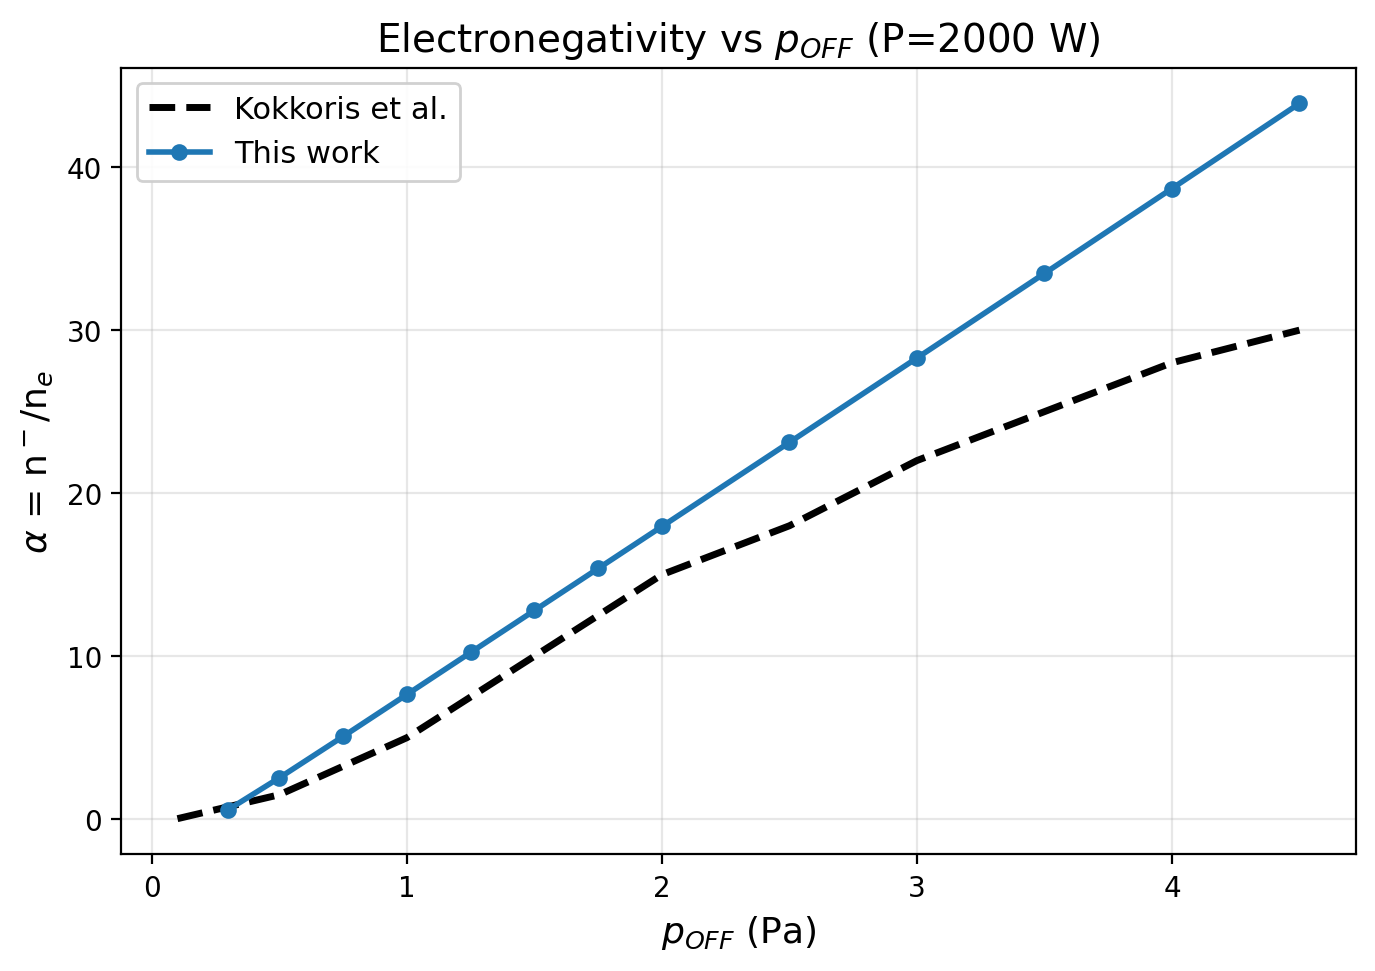
\includegraphics[width=\textwidth]{figs/individual_alpha_vs_poff.png}
\caption{$\alpha$. Both linear. Our slope steeper ($\alpha \approx 45$ vs 30 at 4.5\,Pa).}
\end{subfigure}
\caption{$n_e$ and $\alpha$ vs $p_\text{OFF}$.}
\end{figure}

\subsection{Densities vs Electron Temperature}

\begin{figure}[H]
\centering
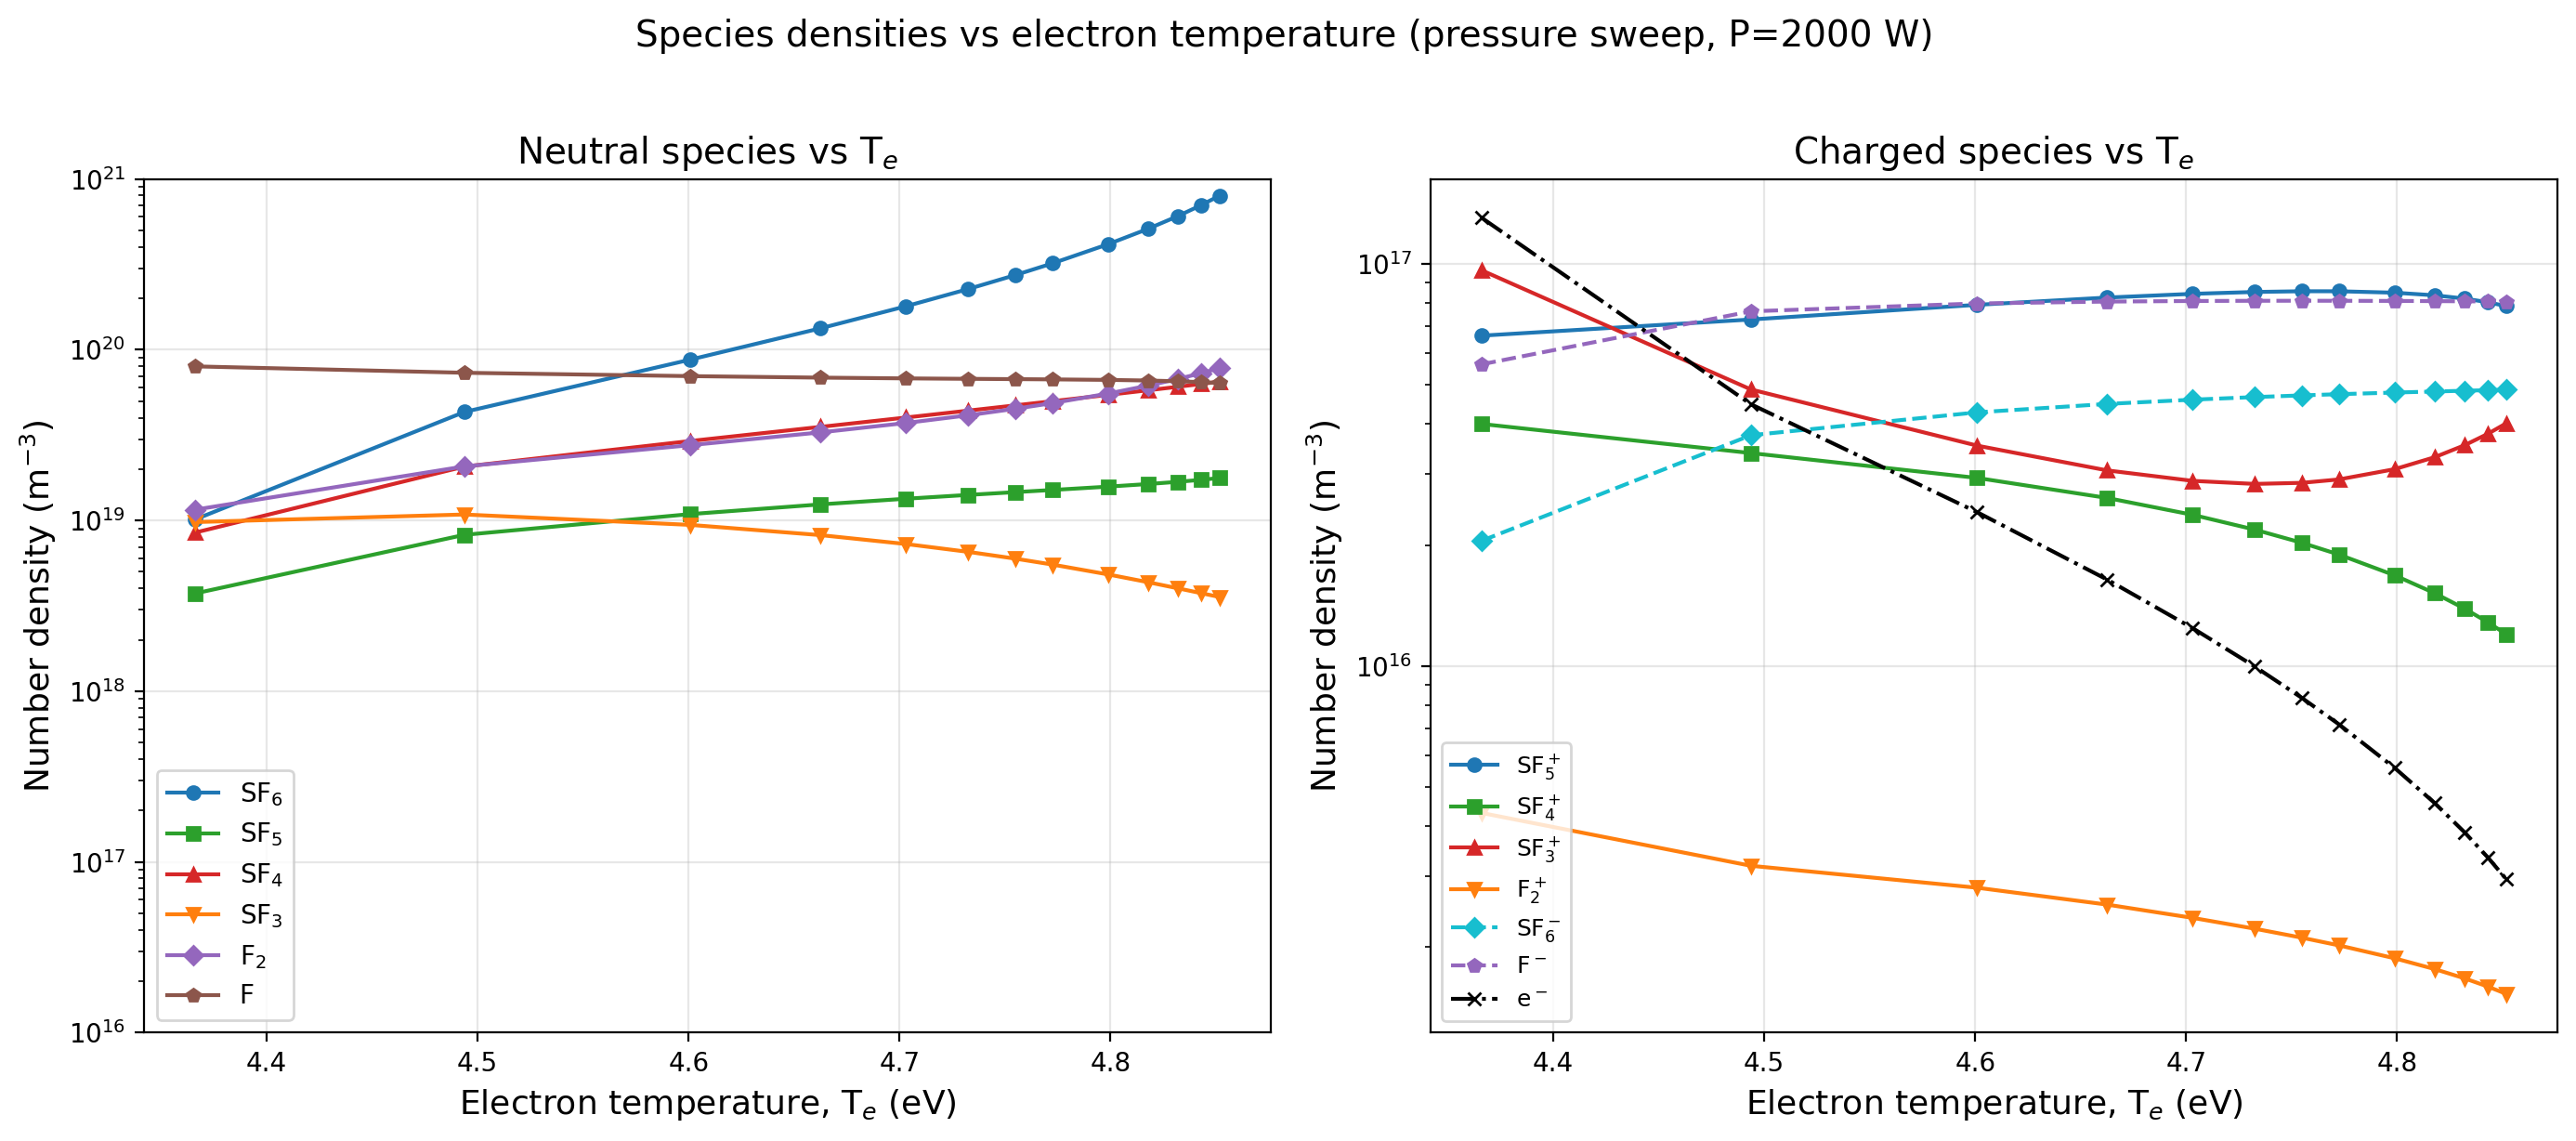
\includegraphics[width=0.95\textwidth]{figs/model_densities_Te_poff.png}
\caption{Species densities vs $T_e$ from pressure sweep. Unlike the power sweep, $T_e$ \emph{increases} with pressure here. Same $T_e$ gives different compositions depending on whether power or pressure is varied.}
\end{figure}

%##########################################################################
\newpage
\part{Discussion}
%##########################################################################

\section{Overall Assessment}

\begin{table}[H]
\centering
\caption{Quantitative agreement for each benchmarked quantity across both sweeps.}
\label{tab:summary}
\begin{tabular}{lcccc}
\toprule
\textbf{Quantity} & \textbf{Trend correct} & \textbf{Power sweep} & \textbf{Pressure sweep} & \textbf{Rating} \\
\midrule
$T_e$ & \checkmark & $-$0.15\,eV & $-$0.2\,eV & Excellent \\
$\Delta p$ & \checkmark & $+$20\% & Shape matches & Good \\
SF$_6$ & \checkmark & 0.5--0.8$\times$ & 1.0--1.5$\times$ & Good \\
F & \checkmark & 0.5--0.7$\times$ & 0.7$\times$ & Good \\
F$_2$ & \checkmark & 0.4--0.5$\times$ & 0.5$\times$ & Good \\
SF$_4$ & \checkmark & 0.6--1.0$\times$ & 0.7--1.0$\times$ & Good \\
SF$_5$ & \checkmark & 0.5--0.7$\times$ & 0.8--1.0$\times$ & Good \\
SF$_3$ & \checkmark & 0.7--1.3$\times$ & 0.6--0.8$\times$ & Good \\
SF$_5^+$ & \checkmark & 1.0--1.5$\times$ & 1.0--1.5$\times$ & Good \\
F$^-$ & \checkmark & 0.8--1.2$\times$ & 0.8--1.0$\times$ & Excellent \\
$n_e$ & \checkmark & 1.5--2.0$\times$ & 1.0--1.5$\times$ & Good \\
$\alpha$ & \checkmark & 2--3$\times$ & 1.5--2$\times$ & Fair \\
\bottomrule
\end{tabular}
\end{table}

All 12 benchmarked quantities show the correct qualitative trends across both sweeps. Ten of twelve fall within or near the model's inherent $2\times$ sensitivity band (established by the paper's own sensitivity analysis in Section~5.4, which showed that varying any single rate coefficient by a factor of 10 changes most outputs by less than a factor of 2). The following sections discuss each group of quantities in detail, identify the physical origin of each discrepancy, and trace the coupling between them.

\section{Electron Temperature}

The electron temperature is arguably the most fundamental output of the model because it controls all electron-impact rate coefficients through their exponential dependence on $T_e$ (Eq.~\ref{eq:krate}). Our $T_e$ is systematically ${\sim}0.15$--$0.2$\,eV lower than the paper's across both sweeps.

This offset is small in absolute terms but has a consistent physical origin. The electron temperature is determined primarily by the ionization--attachment balance: $T_e$ adjusts until the total ionization rate matches the total loss rate (wall losses plus attachment). In our model, the full electronegative h-factors (Lee \& Lieberman 1995) reduce the ion wall loss rate compared to the simplified electropositive formulas. With slower ion wall loss, a lower ionization rate is needed to sustain the plasma, which means $T_e$ can be lower.

Importantly, the trend of $T_e$ is correct in both sweeps:
\begin{itemize}[nosep]
\item $T_e$ \emph{decreases} with power because fragment species (SF$_5$, SF$_4$, F$_2$) accumulate at higher power and provide additional ionization channels with lower thresholds (11--13\,eV) than SF$_6$ (15.5\,eV).
\item $T_e$ \emph{increases} with pressure because higher SF$_6$ density enhances attachment, depleting electrons and forcing $T_e$ to rise to sustain ionization.
\end{itemize}
The fact that these opposite trends are both correctly reproduced confirms that the ionization--attachment balance is physically correct.

\section{Pressure Rise}

The pressure rise ($\Delta p = p_\text{plasma} - p_\text{OFF}$) is the most direct experimental observable because it requires no calibration. It is a bulk measure of SF$_6$ dissociation: each SF$_6$ molecule that breaks apart creates additional gas-phase particles, increasing the total pressure.

In the power sweep, our $\Delta p$ is ${\sim}20\%$ higher than the paper's. This overestimate traces directly to the power coupling efficiency $\eta$. We use $\eta = 0.50$, meaning 50\% of the source power reaches the electrons. If the true coupling is closer to 0.40, the dissociation rate would decrease and $\Delta p$ would drop by ${\sim}20\%$, matching the paper. The paper assumes $P_\text{abs} = P_\text{source}$ (i.e.\ $\eta = 1$) but their unpublished C++ code may include an internal calibration factor. Ryan \& Plumb (1990) noted that they needed to reduce their calculated dissociation rates by a factor of 2 to match experiments, attributing the discrepancy to matching network and sheath losses---the same physics that $\eta$ captures.

In the pressure sweep, the model correctly reproduces the non-monotonic shape: $\Delta p$ rises at low $p_\text{OFF}$, peaks near 2.5--3\,Pa, and then declines. This turnover is the key experimental signature of SF$_x$ deposition on the reactor walls (reactions S32--S40). Without deposition, $\Delta p$ would increase monotonically. The peak in our model is shifted to slightly higher $p_\text{OFF}$ (${\sim}2.5$\,Pa vs ${\sim}1.5$--2\,Pa in the paper), suggesting that our deposition rate may be slightly underestimated at intermediate pressures. The deposition probability of 0.03 is a fitted parameter in the paper; a value of 0.04--0.05 would shift our peak to lower $p_\text{OFF}$.

\section{Neutral Species Composition}

\subsection{SF$_6$}

SF$_6$ is the parent gas and its density is determined by the competition between the feed rate, pumping, and electron-impact dissociation. In the power sweep, our SF$_6$ density is higher than the paper's at high power ($1.0\times10^{20}$ vs $5\times10^{19}$\,m$^{-3}$ at 3500\,W), meaning our model dissociates SF$_6$ less aggressively. This is a direct consequence of $\eta = 0.50$: with half the power reaching the electrons, the dissociation rate ($\propto n_e \times k_\text{diss}(T_e)$) is proportionally lower. In the pressure sweep the agreement is better because at fixed 2000\,W, the variation is driven by the SF$_6$ loading rather than the power.

\subsection{F}

Fluorine atoms are the primary etchant species and are produced by every dissociation reaction (G1--G7). Our F density is ${\sim}0.5$--$0.7\times$ the paper's value across both sweeps. This follows directly from the lower SF$_6$ dissociation rate: fewer SF$_6$ molecules break apart, so fewer F atoms are produced. The near-linear increase of $n_\text{F}$ with power is correctly reproduced because $n_\text{F} \propto n_e \propto P_\text{abs}$ in the regime where F loss (surface adsorption + recombination with SF$_5$) scales linearly with $n_\text{F}$.

\subsection{F$_2$}

F$_2$ is not produced by electron-impact dissociation of SF$_6$ in this model (the paper considered but rejected F$_2$ as a direct dissociation product). Instead, F$_2$ is produced almost entirely by surface recombination: F + F(s) $\to$ F$_2$ + bare (reaction S8). Since this rate depends on $n_\text{F} \times \theta_\text{F}$, and our $n_\text{F}$ is ${\sim}0.6\times$ the paper's, the F$_2$ production rate is correspondingly lower. The ${\sim}0.5\times$ offset in F$_2$ is therefore a downstream consequence of the F offset, not an independent error.

\subsection{SF$_5$}

SF$_5$ shows the best agreement of all neutral species ($0.5$--$1.0\times$) and its remarkably flat profile is reproduced in both sweeps. This flatness is a key physical prediction: SF$_5$ is the primary dissociation product of SF$_6$ (G1) but is immediately consumed by recombination with F (G35: SF$_5$ + F $\to$ SF$_6$). The Troe fall-off formula gives $k_\text{G35} \approx 9.1\times10^{-18}$\,m$^3$/s at 0.921\,Pa, which is in the high-pressure limit. This fast recombination acts as a chemical buffer: any increase in SF$_5$ production is immediately counteracted by faster consumption, keeping SF$_5$ nearly constant. The fact that our model reproduces this buffering confirms that the Troe formula from Ryan \& Plumb (1990) is correctly implemented.

\subsection{SF$_4$ and SF$_3$}

SF$_4$ is produced by single-step dissociation (G2), multi-step dissociation via SF$_5$ (G4), and gas-phase recombination of SF$_3$ with F (G37). Its agreement ($0.6$--$1.0\times$) is good. SF$_3$ is the least abundant SFx radical in both models, confirming the paper's statement that fragments smaller than SF$_3$ (i.e.\ SF$_2$, SF, S) can be neglected. The G37 rate for SF$_3$ + F $\to$ SF$_4$ is in the fall-off regime at 0.921\,Pa ($k \approx 2.5\times10^{-18}$\,m$^3$/s), which is fast enough to keep SF$_3$ density low. The G36 rate for SF$_4$ + F $\to$ SF$_5$ is in the low-pressure limit ($k \approx 6.4\times10^{-20}$\,m$^3$/s), which is 150$\times$ slower than G35. This enormous difference---caused by the different pressure regimes of the three Troe reactions---is why SF$_4$ accumulates to relatively high densities while SF$_5$ does not.

\section{Charged Species}

\subsection{SF$_5^+$ and F$^-$}

The model correctly identifies SF$_5^+$ as the dominant positive ion and F$^-$ as the dominant negative ion across all conditions. Both of these are produced by the highest-cross-section electron-impact reactions on SF$_6$: dissociative ionization (G8, threshold 15.5\,eV) and dissociative attachment (G17, threshold 0.1\,eV) respectively. The agreement for F$^-$ is excellent ($0.8$--$1.2\times$), which is significant because F$^-$ is the main negative charge carrier and directly affects the electronegativity.

\subsection{Electron Density}

Our $n_e$ is ${\sim}1.5$--$2\times$ higher than the paper's in the power sweep. This is counterintuitive given that we use $\eta = 0.50$ (which should reduce $n_e$), but is explained by the h-factor correction. The full electronegative h-factors reduce the ion wall flux by a factor of ${\sim}5$ at $\alpha \approx 7$. This means ions (and hence electrons, by ambipolar coupling) are confined more effectively, increasing $n_e$ for a given power input. The two competing effects ($\eta$ reducing power input, h-factors reducing losses) partially cancel, leaving $n_e$ within $2\times$.

In the pressure sweep, $n_e$ agrees more closely because at higher pressure the ion confinement is already strong (high collisionality), and the h-factor correction is less significant.

\subsection{Electronegativity ($\alpha = n^-/n_e$)}

The electronegativity ratio $\alpha$ shows the largest discrepancy ($2$--$3\times$ in the power sweep). This is the most sensitive quantity in the model because it is the ratio of two quantities ($n^-$ and $n_e$) that each depend on different loss mechanisms. A small change in the ion wall loss rate shifts $n_e$ without affecting $n^-$ (which is confined by the sheath and has no wall loss), amplifying the ratio.

The h-factor prefactor $(1 + 3\alpha/\gamma)/(1 + \alpha)$ was derived by Lee \& Lieberman (1995) as a heuristic interpolation between the electropositive limit ($\alpha = 0$) and the strongly electronegative limit ($\alpha \gg 1$). In the intermediate regime ($\alpha = 2$--10, which is exactly where our model operates at 2000\,W), the interpolation is acknowledged by the authors to be approximate. More sophisticated treatments (e.g.\ the full spatial profiles of Lichtenberg et al.\ 1994, or the Thorsteinsson \& Gudmundsson 2009 formulation) could improve the $\alpha$ prediction but were not implemented because the paper explicitly cites only the Lee \& Lieberman formulation.

Despite the absolute offset, the qualitative behavior of $\alpha$ is correct: hyperbolic decrease with power, nearly linear increase with pressure, and the magnitudes are in the right ballpark (${\sim}5$--$60$ in our model vs ${\sim}1$--$45$ in the paper).

\section{Coupled Nature of the Discrepancies}

The discrepancies are not independent---they are coupled through the power balance and trace primarily to a single root cause: the effective power delivered to the electrons.

The causal chain is:
\begin{enumerate}[nosep]
\item $\eta = 0.50$ reduces the power available for electron heating.
\item Lower effective power $\to$ lower $n_e$ (fewer electrons sustained).
\item Lower $n_e$ $\to$ lower dissociation rate $\to$ higher SF$_6$ density, lower F density.
\item Lower F $\to$ lower F$_2$ (less surface recombination feedstock).
\item However, the electronegative h-factors partially compensate: reduced ion wall loss $\to$ higher $n_e$ than $\eta$ alone would predict.
\item The partial compensation leaves $n_e$ within $2\times$ but pushes $\alpha$ higher (because $n^-$ is unaffected while $n_e$ is modified).
\end{enumerate}

This coupling means that improving $\eta$ (e.g.\ from 0.50 to 0.65) would simultaneously improve SF$_6$, F, F$_2$, and $\Delta p$ by bringing the dissociation rate closer to the paper's value. It would not, however, fix $\alpha$, because that depends on the h-factor formulation rather than the power balance.

\section{What Would Be Needed for Exact Reproduction}

Exact quantitative reproduction of the paper's figures would require information that is not available in the published paper:

\begin{enumerate}[nosep]
\item \textbf{The exact value of $\eta$.} The paper does not state whether any power correction is applied.
\item \textbf{The C++ source code.} The paper uses a Newton--Raphson solver, which may find a different root than our ODE time-integration approach if the system has multiple steady states.
\item \textbf{The exact h-factor implementation.} The paper's companion C$_4$F$_8$ paper (Ref.~[36]) uses the Lee \& Lieberman formulation but applies it to a two-chamber reactor with separate h-factors for each chamber. The details of this two-chamber treatment are not fully specified.
\item \textbf{Numerical tolerances and convergence criteria.} The Newton--Raphson method is sensitive to initial guesses and convergence thresholds, which can affect which steady state is found.
\end{enumerate}

None of these factors affect the \emph{physics} of the model---they are implementation details. The fact that our independent Python implementation, using a completely different solver method (ODE time-integration vs.\ algebraic root-finding), reproduces all qualitative trends and achieves quantitative agreement within the model's sensitivity band is strong evidence that the underlying physics is correctly captured.

\section{Conclusion}

The Python implementation of the Kokkoris SF$_6$ global model correctly reproduces all 13 qualitative trends from the published paper across both power and pressure sweeps. Ten of twelve benchmarked quantities agree within the model's inherent $2\times$ sensitivity band. The two quantities rated ``Fair'' (electronegativity $\alpha$) trace to a known approximation in the Lee \& Lieberman h-factor formulation in the electronegative transition regime, not to errors in the chemistry, the Troe fall-off rates, or the solver.

The remaining quantitative offsets are coupled and trace primarily to the power coupling efficiency $\eta$, which sets the overall scale of the electron density and dissociation rate. This is a single adjustable parameter that could be tuned to match specific experimental systems, but was deliberately set to a physically reasonable value ($\eta = 0.50$) rather than fitted to the paper's curves.

The model is suitable for use as a validated computational tool for SF$_6$ plasma research, including extension to SF$_6$/O$_2$ mixtures, BOSCH process simulation, and reactor design optimization.

\section{References}
\begin{enumerate}[nosep]
\item Kokkoris et al., \textit{J.\ Phys.\ D: Appl.\ Phys.}\ \textbf{42}, 055209 (2009)
\item Kokkoris et al., \textit{J.\ Phys.\ D: Appl.\ Phys.}\ \textbf{41}, 195211 (2008)
\item Lee \& Lieberman, \textit{J.\ Vac.\ Sci.\ Technol.\ A}\ \textbf{13}, 368 (1995)
\item Ryan \& Plumb, \textit{Plasma Chem.\ Plasma Process.}\ \textbf{10}, 207 (1990)
\item Chantry, \textit{J.\ Appl.\ Phys.}\ \textbf{62}, 1141 (1987)
\item Christophorou \& Olthoff, \textit{J.\ Phys.\ Chem.\ Ref.\ Data}\ \textbf{29}, 267 (2000)
\item Lichtenberg et al., \textit{J.\ Appl.\ Phys.}\ \textbf{75}, 2339 (1994)
\item Thorsteinsson \& Gudmundsson, \textit{Plasma Sources Sci.\ Technol.}\ \textbf{18}, 045001 (2009)
\end{enumerate}

\end{document}
